%\documentclass[12pt]{exam}

\documentclass[12pt]{article}  
% Эта строка — комментарий, она не будет показана в выходном файле  
\usepackage[russian]{babel}  % Включаем пакет для поддержки русского языка  
\usepackage{ucs} 
\usepackage[utf8x]{inputenc} % Включаем поддержку UTF8  
\usepackage{gensymb}
\usepackage[left=2cm,right=2cm,
    top=1.5cm,bottom=1.5cm,bindingoffset=0cm]{geometry}
\usepackage{titling}   % для удвоения титульной страницы
\usepackage{titlesec}
\titleformat{\part}[block]{\Large\bfseries\flushright\it}{}{1em}{}
\titleformat{\section}[block]{\small\bfseries\filcenter}{}{1em}{}
\titleformat{\subsection}[hang]{\footnotesize\bfseries\filcenter}{}{1em}{}
\titleformat{\subsubsection}[hang]{\footnotesize\bfseries\filcenter}{}{1em}{}
%\usepackage[12pt]{extsizes} % для того чтобы задать нестандартный 14-ый размер шрифта
\usepackage[fontsize=15.5pt]{scrextend}
\usepackage{graphicx}
\usepackage{amstext}
\usepackage{multirow}
\newcommand{\mc}{\multicolumn}
\graphicspath{ {./images/} }
\date{}  
\author{}
\usepackage[pdftex,
            pdfauthor={programmer78@bk.ru},
            pdftitle={user manual},
            pdfsubject={ECON-03},
            pdfkeywords={radio construction kit, user manual, schematic diagrams},
            pdfproducer={Latex with hyperref},
            pdfcreator={pdflatex}]{hyperref}
            
\begin{document}
\title{\vspace{5em}ИГРУШКА\\
\vspace{2em}КОНСТРУКТОР ЭЛЕКТРОННЫЙ\\
ЭКОН-03\\
электронная лаборатория\\
руководство по эксплуатации}\maketitle 
\pagestyle{empty} % нумерация выкл.
\thispagestyle{empty}

\clearpage\mbox{}\clearpage
\newpage

\title{\vspace{5em}ИГРУШКА\\
\vspace{2em}КОНСТРУКТОР ЭЛЕКТРОННЫЙ\\
ЭКОН-03\\
электронная лаборатория\\
руководство по эксплуатации}\maketitle 
\pagestyle{empty} % нумерация выкл.
\thispagestyle{empty}
\newpage
\vspace*{360px}
\textsuperscript{\textcopyright} ВНИИ <<Электронстандарт>>, 1987
\\
\\
\\
Ответственный редактор Г.С.Стерин

Редактор В.В. Новикова

Технический редактор Н.Е.Меркурьева Корректор Л.И.Иванова

\hrulefill

{\small
Сдано в набор 26/XII-86 г. \hspace{1em} Подписано к печати 23/I-87 г. \hspace{1em} Печ. л. 5 п.л.

Уч.-изд. л. 4,8 \hspace{1em} Бесплатно \hspace{4em} Изд. № 478 \hspace{8em} Зак. 800}

\hrulefill

Документ свёрстан в системе \LaTeX{} в 2019 году по оригиналу 1987 года \href{https://vk.com/programmer78}{programmer78@bk.ru}

\newpage
\pagestyle{plain} % нумерация вкл.
\setcounter{page}{3} % начать нумерацию с номера три
\vspace*{7em}
\section{ОБЩИЕ УКАЗАНИЯ}
Игрушка конструктор электронный <<Экон-03>>, которая в дальнейшем будет называться конструктор, предназначена для технического творчества в области радиоэлектроники начинающих радиолюбителей и детей в возрасте 13 лет и старше.

Конструктор позволяет без применения пайки и инструкмента с помощью монтажных проводов производить сборку различных действующих электронных устройств.

Конструктор рассчитан на эксплуатацию в помещениях при температуре окружающего воздуха от +15 до + 35 \degree C.

При работе с конструктором внимательно ознакомьтесь с настоящим руководством по эксплуатации.

\section{ТЕХНИЧЕСКИЕ ДАННЫЕ}

Габаритные размеры в потребительской таре - не более 430х262х63 мм.

Масса - не более 1,6 кг.

Напряжение источника питания - 9,0 В;

Максимальный ток, потребляемый конструктором, - не более 100 мА.

Продолжительность работы конструктора от одного комплекта свежеизготовленных элементов А316 <<Квант>> при непрерывной работе по 4 ч в сутки должна быть не менее 32 ч.

Количество приведённых в руководстве по эксплуатации электронных устройств - 50.

Предприятие-изготовитель оставляет за собой право вносить в конструктор изменения, не ухудшающие его качества.

\section{КОМПЛЕКТ ПОСТАВКИ}
В комплект поставки входят:
\begin{itemize}
  \setlength\itemsep{-0.2em}
  \item[] конструктор \dotfill 1 шт.
\newpage
  \item[] провод антенный длиной 2 м \dotfill 1 шт.
  \item[] провод длинный \dotfill 4 шт.
  \item[] провод средний \dotfill 18 шт.
  \item[] провод короткий \dotfill 35 шт.
  \item[] элементы А316 <<Квант>> \dotfill 6 шт.
  \item[] руководство по эксплуатации \dotfill 1 шт.
  \item[] потребительская тара \dotfill 1 шт.
\end{itemize}

\section{УСТРОЙСТВО КОНСТРУКТОРА}
Конструктор представляет собой плату 1 с закреплёнными на ней радиоэлектронными элементами 2. Выводы каждого радиоэлектронного элемента пропущены через плату и закреплены в нижней части пружин-контактов 3, с которыми имеют надёжный электрический контакт. Верхняя часть пружины-контакта, находящаяся над платой, является элементом коммутации. Электрические соединения между пружинами-контактами осуществляются проводами 4. Окно фоторезистора закрыто крышкой 5, которая используется для защиты фоторезистора в неработающем состоянии.

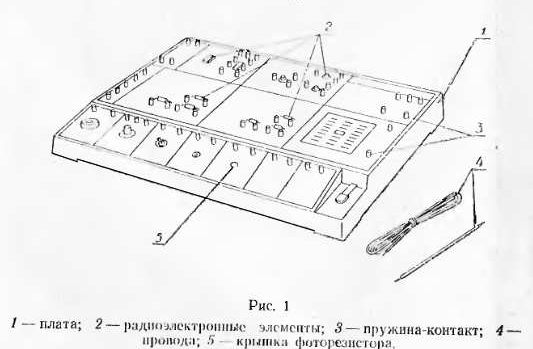
\includegraphics[scale=0.8]{ekon3_004}

Для питания игрушки можо использовать серийно выпускаемые блоки питания с выходным напряжением 9 В: БП-9/60, ПУ-1М, БПС-9/12, БПС 4-12, ВБ-1 и аналогичные.
\newpage
\section{ПОДГОТОВКА К РАБОТЕ}
Перед началом работы с конструктором проверьте годность элементов питания. На элементах не должно быть вздутий и следов утечки электролита. Загрязнённые контакты необходимо зачистить. Если на элементах имеется налёт карбонатов, то перед установкой в конструктор элементы следует протереть сухой тканью.

В домашних условиях при отсутствии измерительных приборов приблизительную оценку качества элементов питания можно производить с помощью электрической лампы для карманного фонаря на 2,5-3,5 В. При работоспособном элементе лампа должна гореть без снижения яркости не менее 15 с.

На отдельных элементах вокруг контактной площадки <<->> бывает сильно выступающий ободок, который препятствует контактированию. Его необходимо подрезать.

Конструктор может работать только при условии, если все шесть элементов А316 исправны.

Претензии по элементам питания направляйте на завод-изготовитель.
Установите элементы в отсек питания конструктора, соблюдая полярность и обеспечивая надёжный контакт, закройте крышку.

БУДЬТЕ ВНИМАТЕЛЬНЫ! НЕПРАВИЛЬНАЯ УСТАНОВКА ЭЛЕМЕНТОВ ПИТАНИЯ ИЛИ ПОДКЛЮЧЕНИЕ БЛОКА ПИТАНИЯ МОЖЕТ ПРИВЕСТИ К ВЫХОДУ ИЗ СТРОЯ СХЕМЫ ЭЛЕКТРИЧЕСКОЙ ПРИНЦИПИАЛЬНОЙ.
\newpage
\section{ПОРЯДОК РАБОТЫ}
Сборка электронных устройств осуществляется по приведённым в руководстве по эксплуатации схемам электрическим принципиальным и таблицам соединений контактов. Собирая электронное устройство, следите за тем, чтобы соединения обеспечивали надёжный электрический контакт. Параметры радиоэлектронных элементов, входящих в состав конструктора, особенно транзисторов, могут значительно отличаться один от другого. Поэтому для улучшения работы некоторых электронных устройств может потребоваться подбор величин сопротивлений резисторов, стоящих в цепи баз транзисторов. Резисторы, на электрических схемах обозначенные *, составлены из нескольких резисторов конструктора.

При сборке усилителей и радиоприёмников необходмо пользоваться проводниками возможно меньшей длины, так акак из-за сложного пространственного монтажа схемы склонны к самовозбуждению - появлению нежелательных звуков (свист, щелчки и т.п.).

Назначение и графическое обозначение радиоэлектронных элементов, входящих в состав конструктора, приведены в приложении 1.

Сборку электронных устройств вдобно производить с помощью таблиц соединений (см. приложение 2).

В первых двух графах таблицы - номера соединяемых контактов, а в третьей - обозначение длины соединительных проводов:\\
Д - длинный;\\
С - средний;\\
К - короткий.

Запись в таблице, например 18-24-К, следует понимать так: контакты-пружины №18 и 24 скоммутировать с помощью короткого провода.

При сборке электронных устройств №44, 55, 56, 63, 66 крышку с фоторезистора снять.

\section{ПРАВИЛА ХРАНЕНИЯ}
Конструктор следует хранить в потребительской таре в отапливаемых и вентилируемых помещениях с температурой воздуха от 10 до 40 \degree C и относительной влажностью $60\pm 10\%$ на расстоянии не менее 1 м от отопительных приборов.

Не рекомендуется длительное хранение конструктора с находящимися в нём батареями питания свыше их гарантийного срока хранения. Это может привести к утечке электролита из батарей и порче радиоэлементов.
\newpage
\part{ПРИЛОЖЕНИЕ 1}
\vspace*{4em}
\section{НАЗНАЧЕНИЕ И ГРАФИЧЕСКОЕ ОБОЗНАЧЕНИЕ РАДИОЭЛЕКТРОННЫХ ЭЛЕМЕНТОВ, ВХОДЯЩИХ В СОСТАВ КОНСТРУКТОРА}

\textbf{Резистор} - радиоэлектронный элемент, обладающий электрическим сопротивлением, т.е. свойством препятствовать прохождению через него электрического тока. В электронных устройствах резисторы используются для обеспечения требуемых напряжений и токов. Единицей измерения сопротивления является ом (Ом). Производные единицы: килоом (кОм), равный 1000 Ом, мегаом (МОм), равный 1000 кОм или 1 000 000 Ом. Резистор, сопротивление которого неизменно, называется постоянным. Обозначение постоянного резистора на схеме электрической принципиальной показано на рис. 2.


\includegraphics[scale=0.8]{ekon3_008_1}

\textbf{Переменный резистор.} Кроме постоянных, существуют резисторы, сопротивление которых можно изменять в определённых пределах вручную. Сопротивление между выводами 1 и 3 у такого резистора постоянно, а между выводами 1 (или 3) и 2 изменяется. Обозначение переменного резистора показано на рис. 3.


\includegraphics[scale=0.8]{ekon3_008_2}

\newpage
\textbf{Фоторезистор} - это такой радиоэлектронный элемент, сопротивление которого изменяется под воздействием внешней освещённости. Обозначение фоторезистора показано на рис. 4.


\includegraphics[width=\textwidth]{ekon3_009_1}

\textbf{Конденсатор} - радиоэлектронный элемент, обладающий электрической ёмкостью, т.е. свойством накапливать электрический заряд. Конденсатор не пропускает постоянный ток, а переменному оказывает сопротивление тем меньше, чем больше частота тока и ёмкость конденсатора. Обозначение конденсатора показано на рис. 5ф. На рис. 5б показано обозначение электролитического конденсатора.


\includegraphics[width=\textwidth]{ekon3_009_2}

Электролитический конденсатор можно подключать к источнику напряжения только при соблюдении полярности, иначе он выйдет из строя. На электрических схемах обязательно указывается полярность электролитического конденсатора.

Единица измерения электрической ёмкости - фарада (Ф). В качестве производных единиц ёмкости в радиотехнике и электронике приняты микрофарада (мкФ) - одна миллионная часть фарады и пикофарада - одна миллионная часть микрофарады.

\textbf{Конденсатор переменной ёмкости.} Кроме рассмотренных конденсаторов, существуют такие, ёмкость которых можно изменять. Чаще всего изменение ёмкости осуществляется за счёт изменения площади взаимного перекрытия роторных
\newpage
(подвижных) и статорных (неподвижных) пластин. Обозначение конденсатора переменной ёмкости показано на рис. 6.


\includegraphics[scale=0.8]{ekon3_010_1}

\textbf{Катушка индуктивности.} Индуктивность количественно характеризует индукцию, т.е. свойство элемента электрической цепи препятствовать всякому изменению протекающего по нему тока. Катушка индуктивности оказывает переменному току сопротивление, которое тем больше, чем выше частота тока и чем больше индуктивность. При неизменном количестве витков индуктивность можно увеличить, если в катушку ввести сердечник из специального магнитного материала.

Единицей измерения индуктивности является генри (Гн). В качестве производных единиц используются миллигенри (мГн) - одна миллионная часть генри и микрогенри (мкГн) - одна тысячная часть миллигенри. Обозначение катушки индуктивности показано на рис. 7.


\includegraphics[scale=0.8]{ekon3_010_2}

В конструкторе катушки индуктивности используются в ферритовой антенне, обозначение которой показано на рис.8, и трансформаторах низкой частоты, рис.9.

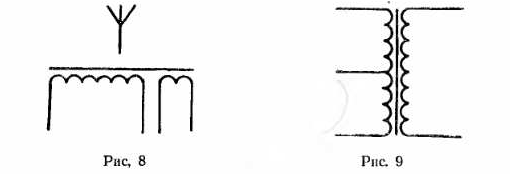
\includegraphics[scale=0.8]{ekon3_010_3}

\newpage
\textbf{Полупроводниковый диод} - это радиоэлектронный элемент, обладающий односторонней проводимостью электрического тока. Диод имеет два электрода: катод - отрицательный и анод - положительный. Катодом служит полупроводник n-типа, а анодом - полупроводник p-типа. Между полупроводниками n- и p-типов образуется p-n-переход. Обозначение полупроводникового диода показано на рис.10.


\includegraphics[scale=0.8]{ekon3_011_1}

\textbf{Светодиод} - полупроводниковый прибор, способный излучать свет при подключении его к источнику тока. Нормальный режим работы светодиода обеспечивается последовательным подключением с ним резистора. Обозначение светодиода показано на рис. 11.


\includegraphics[scale=0.8]{ekon3_011_2}

\textbf{Транзистор} - радиоэлектронный элемент, способный усиливать и генерировать электрические колебания. Области полупроводника, образующего p-n-переходы, называются эмиттер (Э), база (Б) и коллектор (К). Управляющее напряжение прикладывается к переходу Э-Б транзистора. В зависимости от того, какую проводимость имеют эмиттер, база и коллектор, транзисторы могут быть p-n-p- и n-p-n-типов. Обозначение транзисторов p-n-p- и n-p-n- типов показано на рис. 12, а и б соответственно.


\includegraphics[scale=0.8]{ekon3_011_3}

\newpage

\textbf{Микросхема.} Развитие технологии позволило получать в кристалле полупроводника не только диоды и транзисторы, но и резисторы и конденсаторы небольшой ёмкости. Причём количество деталей в единице объёма стало очень большим.

Микросхема, входящая в состав конструктора, представляет собой двухкаскадный усилитель на двух транзисторах структуры n-p-n. Её схема показана на рис.13, а графическое изображение на схемах электрических принципиальных электронных устройств - на рис. 14.

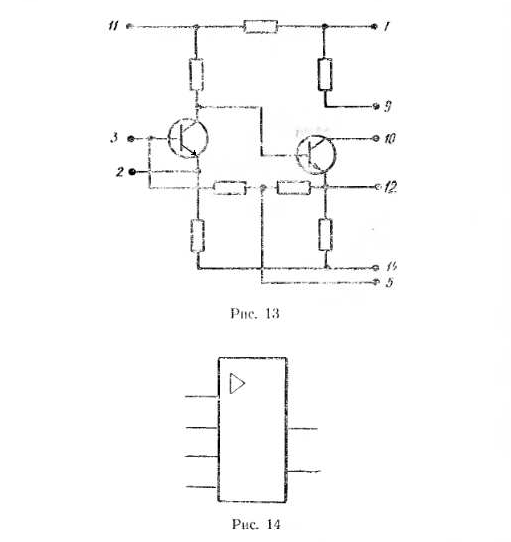
\includegraphics[scale=0.87]{ekon3_013_1}

Для удобства самостоятельной сборки электронных устройств ниже приводится таблица, в которой показано, как подключаются выводы микросхем к контактам конструктора.

\newpage

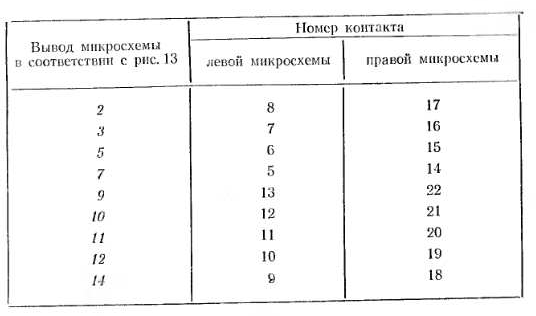
\includegraphics[scale=0.85, angle=-1]{ekon3_012_1}

\textbf{Реле электромагнитное} представляет собой геркон, установленный внутри катушки индуктивности. Под действием электромагнитного поля, образующегося вокруг катушки при прохождении по ней электрического тока, геркон срабатывает и замыкает электрическую цепь. Обозначение реле показано на рис. 15.


\includegraphics[scale=0.85]{ekon3_012_2}

\textbf{Головка громкоговорителя динамическая} является преобразователем электрической энергии в звуковую. В магнитном поле сильного постоянного магнита находится катушка, связанная с диффузором. При прохождении через катушку электрического тока вокруг неё образуется своё магнитное поле, которое взаимодействует с полем магнита. В результате взаимодействия происходит перемещение катушки. Величина и направление перемещения зависят от величины и направления протекающего по катушке тока. Поскольку диффузор связан с катушкой, он также совершает движение, вызывая тем самым колебания воздуха, т.е. образуя звуковые волны. Обо-
\newpage

значение головки громкоговорителя динамической на схеме показано на рис.16.


\includegraphics[width=\textwidth]{ekon3_014_1}

Для улучшения акустических данных головки её обычно помещают в корпус. Система, состоящая из корпуса и находящейся в нём динамической головки, называется громкоговорителем.

\textbf{Источник тока.} В конструкторе в качестве источников тока используются батареи гальванических элементов.

Элемент устроен таким образом, что в результате химической реакции на одном его электроде скапливаются отрицательно заряженные ионы, образуя отрицательный электрод элемента, а на другом - положительно заряженные ионы, образуя положительный электрод элемента. Поскольку электродвижущая сила (ЭДС) одного элемента невелика, элементы соединяют в батарею, получая необходимую величину ЭДС.

В качестве единицы измерения электрического напряжения принят вольт (В). Для простоты обозначения очень больших или очень малых напряжений установлены производные единицы. Так, тысяча вольт называется киловольтом (кВ), одна тысячная часть вольта - милливольтом (мВ), миллионная часть вольта - микровольтом (мкВ). Обозначение батареи гальванических элементов показано на рис. 17.


\includegraphics[width=\textwidth]{ekon3_014_2}

\textbf{Ключ} служит для кратковременного замыкания электрической цепи. При нажатии ключа электрическая цепь замыкается, при отпускании - размыкается (рис.18).


\includegraphics[scale=0.9]{ekon3_014_3}

\newpage

\part{ПРИЛОЖЕНИЕ 2}
\section{СХЕМЫ ЭЛЕКТРИЧЕСКИЕ ПРИНЦИПИАЛЬНЫЕ ЭЛЕКТРОННЫХ УСТРОЙСТВ И ТАБЛИЦЫ СОЕДИНЕНИЙ КОНТАКТОВ}

\subsection{ЗАКОН ОМА}

При замыкании электродов источника тока проводником электроны с отрицательно заряженного электрода устремляются к положительно заряженному. В проводнике возникает электрический ток. За направление электрического тока принято направление движения положительно заряженных частиц к отрицательному электроду источника тока. Очевидно, что величина электрического тока I будет зависеть от напряжения между электродами U и сопротивления проводника R, соединяющего электроды.

Зависимость между величинами I, U и R была сформулирована в виде закона Ома. Математически закон выражается так:

\begin{equation}
I = \frac{U}{R}
\label{Ohm_law1}
\end{equation} 

откуда можно получить

\begin{equation}
U = R I
\label{Ohm_law2}
\end{equation} 

\begin{equation}
R = \frac{U}{I}
\label{Ohm_law3}
\end{equation} 

\subsection{ПОСЛЕДОВАТЕЛЬНОЕ И ПАРАЛЛЕЛЬНОЕ ВКЛЮЧЕНИЕ ПОТРЕБИТЕЛЕЙ ТОКА}

В цепи, изображённой на рис. 19а, нагрузкой источника тока являются соединённые последовательно резистор сопротивлением 750 Ом и светоизлучающий диод, сопротивление которого не учитывается. Если в разрыв этой цепи включить дополнительно резистор сопротивлением 1,5 кОм (рис. 19б), можно заметить, что свечение светодиода становится меньше,

\newpage

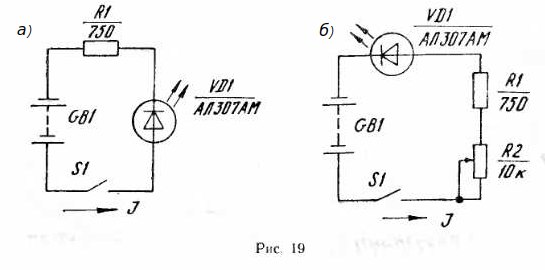
\includegraphics[scale=0.9]{ekon3_016_1}

\hspace{2em}\begin{tabular}{rcrcr}
86  & - & 120 & - & K\\
87  & - & 123 & - & K\\
119 & - & 124 & - & K\\
\end{tabular}
\hspace{10em}\begin{tabular}{rcrcr}
86  & - & 119 & - & K\\
87  & - &  90 & - & K\\
91  & - & 124 & - & K\\
120 & - & 123 & - & K\\
\end{tabular}

При последовательно соединении общее сопротивление цепи равно сумме составляющих её сопротивлений:

\begin{equation}
R = R1 + R2 + ... + RN.
\label{Ohm_series}
\end{equation}

В первом случае

$$ R' = R1; $$

Во втором случае

$$ R'' = R1 + R2. $$

Зная напряжение источника тока и сопротивление цепи, по формуле (\ref{Ohm_law1}) можно расчитать ток в цепи.

В первом случае $$ I' = \frac{U}{R'} = \frac{U}{R1}; $$

во втором случае $$ I'' = \frac{U}{R''} = \frac{U}{R1+R2}. $$


\newpage

С помощью переменного резистора R1 установим слабое свечение светодиода (рис. 20). При нажатии на ключ S1 параллельно резистору R1 подключается резистор R2. При этом яркость свечения светодиоа заметно выше. При параллельном соединении элементов цепи общее сопротивление уменьшается:

\begin{equation}
R = \frac{R1 R2}{R1 + R2}
\label{Ohm_parallel}
\end{equation}

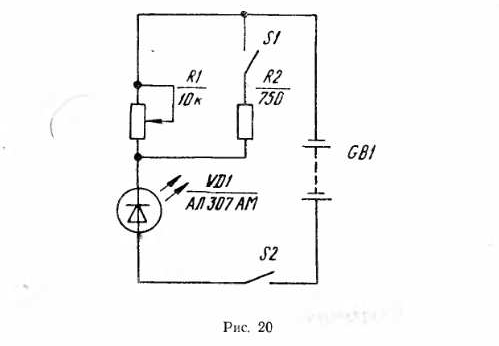
\includegraphics[scale=0.9]{ekon3_017_1}

\hspace{1cm}\begin{tabular}{rcrcrp{3cm}rcrcr}
86   & - & 116 & - & C &   & 116 & - & 120 & - & C\\
87   & - & 126 & - & C &   & 117 & - & 119 & - & K\\
114  & - & 115 & - & K &   & 118 & - & 124 & - & C\\
115  & - & 125 & - & Д &   & 123 & - & 125 & - & K\\
\end{tabular}

Общее сопротивление параллельно включаемых сопротивлений меньше меньшего сопротивления.

\subsection{ПЕРЕМЕННЫЙ ТОК}

Всякий ток, изменяющийся с течением времени по величине и направлению, является переменным.
\newpage
На рис. 21 показан график тока, который изменяется периодически по гармоническому закону.

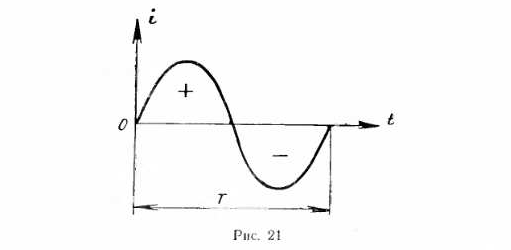
\includegraphics[width=\textwidth]{ekon3_018_1}

Весь цикл измененеия тока соответствует одному периоду колебаний Т. Период колебаний - это время, в течение которого ток проходит через все промежуточные значения и возвращается к произвольно выбранному исходному значению. Число таких изменений, происходящих в секунду, называется частотой и обозначается буквой f.

\begin{equation}
f = \frac{1}{T}
\end{equation}

Частота выражается в герцах (Гц) или его производных единицах - килогерцах (кГц) и мегагерцах (МГц). Один килогерц равен тысяче герц, т.е.. 1 кГц = 1000 Гц, а один мегагерц равен тысяче килогерц, т.е. 1 МГц = 1000 кГц.

\subsection{УСИЛИТЕЛЬНЫЕ УСТРОЙСТВА}
\subsubsection{Транзистор - усилительный элемент}

В устройстве, электрическая схема которого изображена на рис.22, существует возможность с помощью переменного резистора регулировать ток в цепи базы транзистора. Это влечёт за собой изменение тока в цепи коллектора, о чём можно судить по изменению свечения светодиода.
\newpage

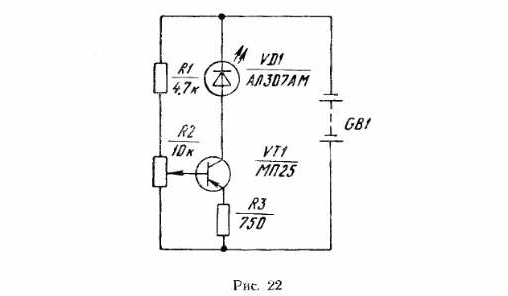
\includegraphics[width=\textwidth]{ekon3_019_1}

\hrulefill

\begin{tabular}{r c r c r p{2cm} r c r c r p{2cm} r c r c r}
27 & - & 115 & - & C &     & 87 & - & 124 & - & C &    & 116 & - & 124 & - & C\\
28 & - & 119 & - & C &     & 94 & - & 114 & - & K &    & 120 & - & 123 & - & K\\
29 & - &  86 & - & K &     & 95 & - & 123 & - & C &    &     &   &     &   &  \\
\end{tabular}

\hrulefill

Данное устройство является простейшим усилителем постоянного тока (УПТ).

\vspace*{13em}
\subsubsection{Схемы включения транзисторов в усилителях}

В зависимости от того, какой электрод транзистора является общим для входной и выходной цепей, различают три схемы включения транзистора: с общим эмиттером (рис.23а), общей базой (рис.23б) и общим коллектором (рис.23в).

\newpage
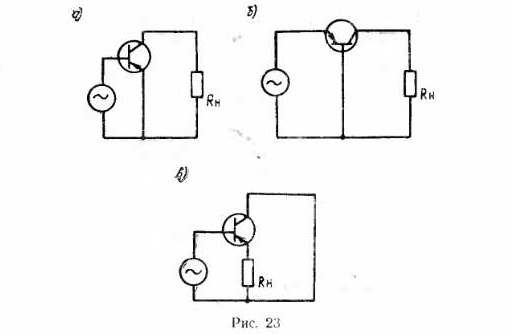
\includegraphics[scale=0.8]{ekon3_020_1}

Считается, что усилительные свойства каскада на транзисторе полностью определены, если известны его входное и выходное сопротивление и коэффициент усиления по току, напряжению и мощности. Сравнивая между собой соответствующие параметры однокаскадного усилителя в различных схемах включения транзистора, можно сделать следующие выводы.

\begin{itemize}
\item[1.] Коэффициент усиления по напряжению в схемах с общим эмиттером и общей базой одинаков, а в схеме с общим коллектором он всегда несколько меньше единицы.
\item[2.] Коэффициент усиления по току в схеме с общим эмиттером и общим коллектором одинаков, а в схеме с общей базой всегда несколько меньше единицы.
\item[3.] Коэффициент усиления по мощности в схеме с общим эмиттером максимален, а в схеме с общим коллектором минимален.
\item[4.] Входное сопротивление в схеме с общим коллектором максимально, а в схеме с общей базой минимально.
\item[5.] Выходное сопротивление в схеме с общей базой максимально, а в схеме с общим эмиттером минимально.
\end{itemize}

Схема с общим эмиттером имеет наибольшее усиление по мощности и средние значения входного и выходного сопротивлений, поэтому она чаще других используется в усилителях.
\newpage
\subsubsection{Однокаскадный усилитель низкой частоты}

Схема однокаскадного усилителя, пригодного для практического применения, приведена на рис. 24

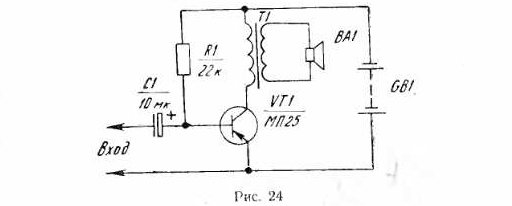
\includegraphics[width=\textwidth, angle=-1]{ekon3_021_1}

\hrulefill

\hspace{1cm}\begin{tabular}{rcrcrp{3cm}rcrcr}
27  & - & 98  & - & C &   & 44 & - & 123  & - & C\\
27  & - & 73  & - & C &   & 47 & - & 110  & - & K\\
28  & - & 46  & - & C &   & 48 & - & 111  &  & К\\
29  & - & 124 & - & C &   & 72 & - & вход &  & \\
44  & - & 99  & - & C &   & 29 & - & вход &  & \\
\end{tabular}

\hrulefill

Кроме транзистора, являющегося усилительным элементом, на схеме электрической изображены другие элементы.

Резистор R1 требуется для создания необходимого для нормальной работы транзистора напряжения между базой и эмиттером - напряжения смещения. Напряжение смещения невелико и составляет 0,2, ... 0,6 В для различных типов транзисторов. Величина резистора R1 подбирается по минимуму искажений выходного сигнала.

Конденсатор C1 служит для разделения по постоянному току усилителя и источника сигнала.

Трансформатор Т1 служит для согласования высокого сопротивления каскада с низким сопротивлением головки громкоговорителя.

Максимальный уровень входного сигнала - 0,5 В.

{\scriptsize Примечание. Для этого и последующих усилителей низкой частоты максимальный уровень входного сигнала указан ориентировочно, так как в большой степени зависит от параметров входящих в конструктор транзисторов, точности подбора сопротивлений в цепях баз транзисторов, степени разряда источников питания.}

\newpage

Рассматриваемый усилитель из-за своей простоты широко применяется в различных электронных устройствах. Однако он обладает рядом существенных недостатков, важнейшим из которых является его низкая температуррная стабильность.

Для увелиения стабильности схему усилителя необходимо изменить так, как это изображено на рис. 25.

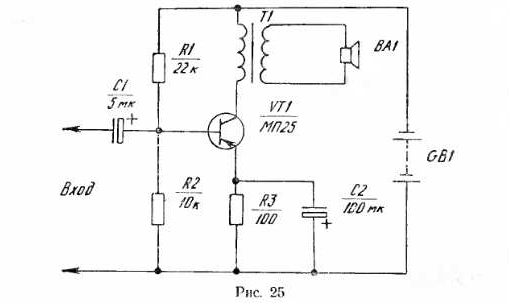
\includegraphics[width=\textwidth]{ekon3_022_1}

\hrulefill

\begin{tabular}{r c r c r p{2cm} r c r c r p{2cm} r c r c r}
27 & - & 71 & - & К &     & 46 & - & 123 & - & C &    &  81 & - &  77  & - & C\\
27 & - & 96 & - & К &     & 46 & - &  99 & - & K &    &  81 & - &  97  & - & K\\
27 & - & 98 & - & С &     & 47 & - & 110 & - & C &    &  97 & - & 124  &   & \\
28 & - & 44 & - & C &     & 48 & - & 111 & - & K &    &  70 & - & вход &   & \\
29 & - & 80 & - & С &     & 80 & - &  76 & - & C &    &  77 &   & вход &   & \\
\end{tabular}

\hrulefill

Резисторы R1, R2 и R3 обеспечивают необходимый режим транзистора по постоянному току и необходимую температурную стабильность усилителя.

Конденсатор С2 служит для устранения отрицательной обратной связи в цепи эмиттера транзистора.

Максимальный уровень входного сигнала - 0,2 В.

\subsubsection{Двухкаскадный усилитель низкой частоты}
Если в схему усилителя, рассмотренного ране, ввести дополнительный каскад предварительного усиления, получится

\newpage
двухкаскадный усилитель, обладающий значительно большей чувствительностью, чем однокаскадный. Каскад предварительного усиления усиливает слабые сигналы до уровня, необходимого для возбуждения усилителя мощности. Схема двухкаскадного усилителя изображена на рис. 26.

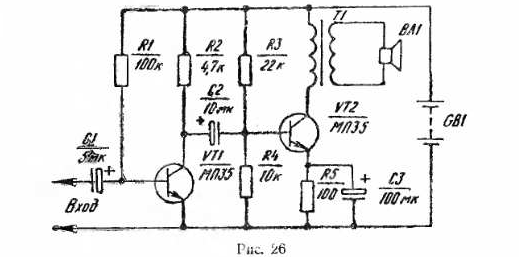
\includegraphics[width=\textwidth]{ekon3_023_1}

\hrulefill

\begin{tabular}{r l r p{0.5cm} r l r p{0.5cm} r l r p{0.5cm} r l r}
30 - & 71  & - К &   & 36 - & 98 & - К &    &  46 - & 124 & - C &   & 77 - & 81  & - К \\
30 - & 104 & - К &   & 36 - & 72 & - С &    &  46 - & 105 & - С &   & 80 - & 96  & - K \\
31 - & 94  & - К &   & 36 - & 97 & - К &    &  47 - & 111 & - К &   & 95 - & 105 & - K \\
31 - & 73  & - C &   & 37 - & 44 & - K &    &  48 - & 110 & - К &   & 95 - & 99  & - K \\
32 - & 96  & - К &   & 38 - & 81 & - C &    &  76 - & 80  & - К &   & 96 - & 123 & - K \\
     &     &     &   &      &    &     &    &       &     &     &   & 70 - & вход &    \\
     &     &     &   &      &    &     &    &       &     &     &   & 76 - & вход &    \\
\end{tabular}

\hrulefill

Сигнал на вход усилителя можно подать с линейного выхода магнитовона или от другого источника с малым уровнем сигнала.

Максимальный уровень входного сигнала - 0,2 В.

\subsubsection{Двухкаскадный усилитель низкой частоты на трёх транзисторах}

Первый каскад усилителя, изображенного на рис. 27, выполнен по схеме составного транзистора. Такое включение транзисторов позволяет получить большое усиление каскада. Режимы работы транзисторов VT1, VT2 и VT3 устанавливаются путём подбора резистора R1 сопротивлением 82-220 кОм. Максимальный уровень входного сигнала 0,1 В. Сигнал на вход усилителя можно подать с линейного выхода магнитофона или от другого источника с малым уровнем сигнала.

\newpage

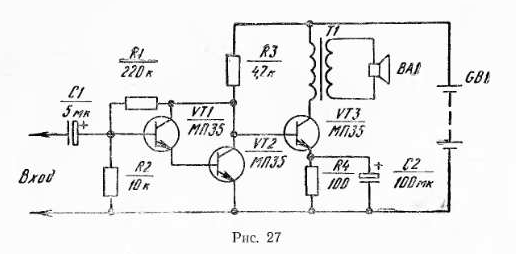
\includegraphics[width=\textwidth]{ekon3_024_1}


\hrulefill

\begin{tabular}{r l r p{0.5cm} r l r p{0.5cm} r l r p{0.5cm} r l r}
30 - & 71  & - К &   & 34 - & 44 & - К &    &  48 - & 110 & - К &   & 107 - & 94   & - К \\
30 - & 96  & - К &   & 35 - & 80 & - С &    &  76 - &  81 & - К &   &  70 - & вход &     \\
31 - & 37  & - К &   & 38 - & 97 & - К &    &  77 - &  80 & - К &   &  76 - & вход &     \\
32 - & 36  & - К &   & 38 - & 81 & - С &    &  95 - & 124 & - К &   &       &      &     \\
33 - & 94  & - К &   & 46 - & 95 & - С &    &  96 - & 106 & - К &   &       &      &     \\
33 - & 37  & - К &   & 47 - &111 & - К &    &  97 - & 123 & - К &   &       &      &     \\
\end{tabular}

\hrulefill

\vspace*{10em}

\subsubsection{Трёхкаскадный усилитель низкой частоты}

На рис. 28 изображена схема трёхкаскадного усилителя с непосредственной связью между двумя последними каскадами. Такое включение позволяет получить хорошую температурную стабильность усилителя и улучшить его характеристики.

Режимы работы транзисторов VT1, VT2 и VT3 устанавливаются подбором резисторов R2 и R4 сопротивлением 82-220 кОм и 220-470 кОм соответственно. Максимальный уровень входного сигнала 0,05 мВ. В качестве источника входного сигнала может быть применён микрофон.
\newpage

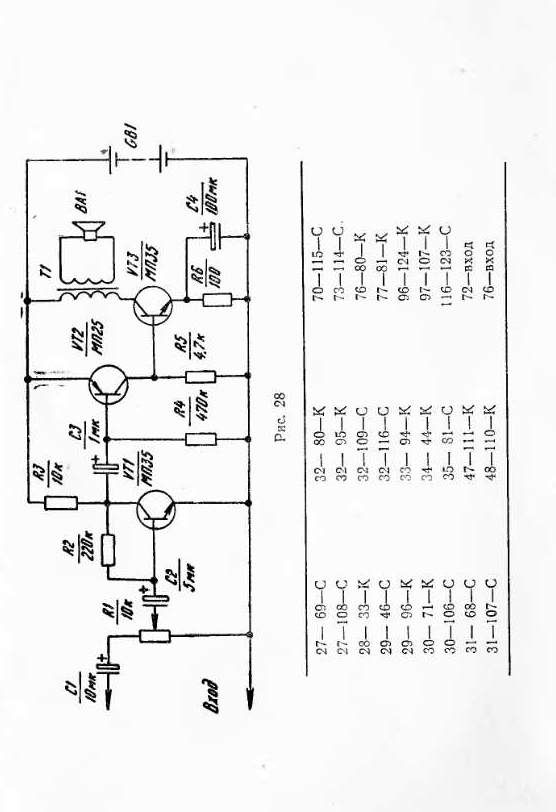
\includegraphics[width=\textwidth]{ekon3_025_1}

\newpage

\subsubsection{Усилитель низкой частоты с использованием микросхемы}

В качестве низкочастотного усилителя может быть использована одна из имеющихся в наборе конструктора микросхем. Эта схема изображена на рис. 29.

Максимальный уровень входного сигнала - 50 мВ.

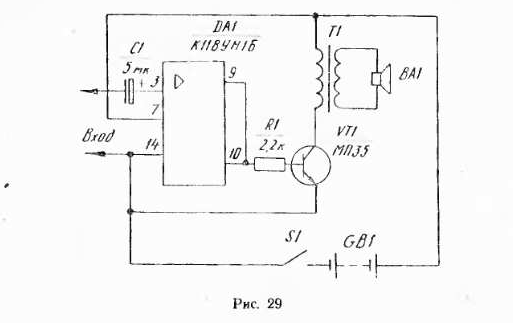
\includegraphics[width=\textwidth]{ekon3_026_1}

\hrulefill

\begin{tabular}{r l r p{0.5cm} r l r p{0.5cm} r l r p{0.5cm} r l r}
14 - & 124  & - С &   & 21 - & 22 & - К &    &  46 - & 124 & - С &   &  18 - & вход & \\
16 - & 71   & - К &   & 21 - & 92 & - С &    &  47 - & 111 & - К &   &  70 - & вход & \\
18 - & 117  & - С &   & 30 - & 93 & - С &    &  48 - & 110 & - К &   &       &      & \\
18 - & 32   & - С &   & 31 - & 44 & - С &    & 118 - & 123 & - К &   &       &      & \\
\end{tabular}

\hrulefill
\vspace*{3cm}
\subsubsection{Усилитель низкой частоты с использованием микросхемы}

В данном усилителе (рис. 30) микросхема использвется в качестве предварительного усилителя. Усилитель мощности выполенен на транзисторе.

Максимальный уровень входного сигнала - 20 мВ. В качестве источника входного сигнала можно использовать микрофон бытового магнитофона.

\newpage

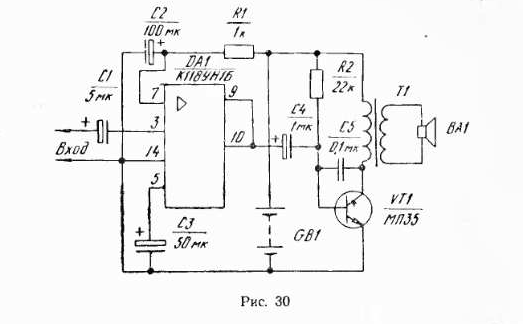
\includegraphics[width=\textwidth]{ekon3_027_1}

\hrulefill

\begin{tabular}{r l r p{0.5cm} r l r p{0.5cm} r l r p{0.5cm} r l r}
14 - & 77  & - С &   & 30 - & 68  & - К &    &  47 - & 111 & - K &   &  66 - & 30 & - C \\
15 - & 75  & - C &   & 30 - & 98  & - С &    &  48 - & 110 & - K &   &  67 - & 31 & - C\\
16 - & 70  & - K &   & 31 - & 44  & - С &    &  74 - & 76  & - K &   &  18 - & вход & \\
18 - & 74  & - C &   & 32 - & 123 & - С &    &  74 - & 123 & - C &   &  71 - & вход & \\
21 - & 22  & - K &   & 46 - & 124 & - С &    &  77 - & 88  & - К &   &       &      & \\
22 - & 69  & - С &   & 46 - & 99  & - С &    &  89 - & 124 & - К &   &       &      & \\
\end{tabular}

\hrulefill

\subsubsection{Двухтактный усилитель мощности}

Во всех ранее рассмотренных низкочастотных усилителях в оконечном каскаде использовался один транзистор. С помощью делителя, включённого в цепь пазы, режим транзистора выбирался таким, что его рабочая точка (Р.Т.) находилась примерно в середине линейного участка характеристики транзистора (рис. 31). В таком усилителе оба полупериода входного гармонического сигнала усиливаются одинаково одним транзистором.

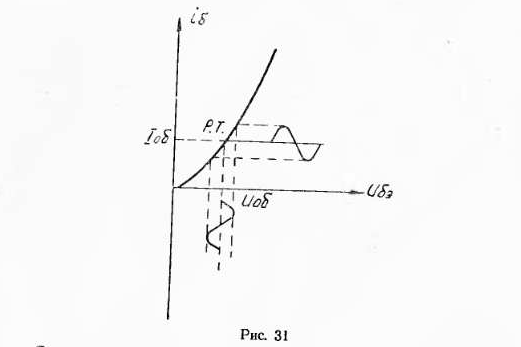
\includegraphics[scale=0.83, angle=2]{ekon3_028_1}

Существенным недостатком таких усилителей является низкий коэффициент полезного действия. Поэтому чаще используются двухтактные усилители мощности.

В таком усилителе для усиления полуволн гармоническго сигнала используются отдельные транзисторы. Транизисторы работают поочерёдно, их рабочие точки на характеристике (рис. 32) выбираются таким образом, что происходит отсечка сигнала.

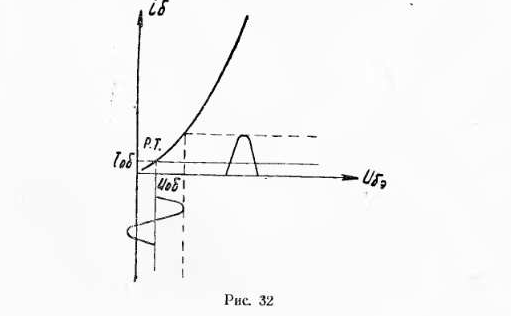
\includegraphics[scale=0.81, angle=1.5]{ekon3_028_2}

\newpage

Для обеспечения работоспособности двухтактного усилителя необходимо на базы составляющих его транзисторов подать сигналы с соотношением фазы одного сигнала по отношению к фазе другого в 180\degree. Для этого может быть изпользован специальный каскад на транзисторе либо трансформатор.

\subsubsection{Двухтактный трансформаторный усилитель}
На рис.33 приведена схема усилителя НЧ, в которой используются два трансформатора. Первый из них, согласующий, обеспечивает подачу на базы транзисторов сигналов в нужной фазе, а второй - для согласования выходного сопротивления транзисторов с сопротивлением головки громкоговорителя.

Максимальный уровень входного сигнала - 10 мВ.

\vspace*{1cm}
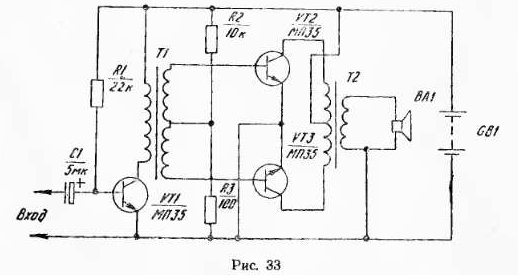
\includegraphics[scale=0.85, angle=1]{ekon3_029_1}
\vspace*{1cm}

\hrulefill

\begin{tabular}{r c r c r p{2cm} r c r c r p{2cm} r c r c r}
30 & - & 71 & - & К &     & 36 & - &  41 & - & К &    &  47 & - & 111  & - & К\\
30 & - & 98 & - & С &     & 38 & - &  47 & - & K &    &  48 & - & 110  & - & K\\
31 & - & 43 & - & С &     & 37 & - &  46 & - & C &    &  42 & - &  99  & - & К\\
32 & - & 38 & - & К &     & 38 & - & 123 & - & С &    &  42 & - & 124  & - & С\\
33 & - & 39 & - & К &     & 40 & - &  96 & - & C &    &  80 & - & 123  & - & С\\
34 & - & 44 & - & К &     & 45 & - &  97 & - & С &    &  81 & - &  96  & - & К\\
35 & - & 38 & - & К &     & 45 & - & 124 & - & C &    &  70 & - & вход &   & \\
   &   &    &   &   &     &    &   &     &   &   &    &  80 & - & вход &   & \\
\end{tabular}

\hrulefill

\newpage

\subsubsection{Двухтактный бестрансформаторный услилитель}

Двухтактный усилитель  может быть построен и по бестрансформаторной схеме. Этот усилитель отличается от предыдущего простотой и отсутствием громоздких трансформаторов (рис. 34).

Максимальный уровень входного сигнала - 1 В.

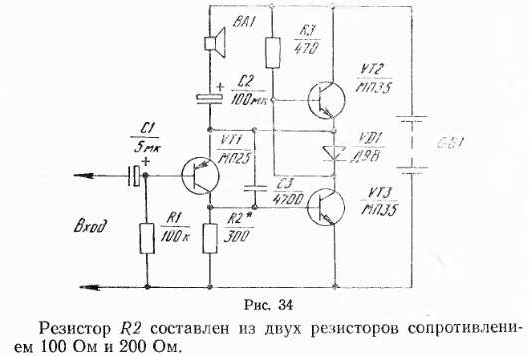
\includegraphics[scale=0.85]{ekon3_030_1}

\hrulefill

\begin{tabular}{r l r p{0.5cm} r l r p{0.5cm} r l r p{0.5cm} r l r}
25 - & 35  & - C &   & 33 - & 37  & - К &    &  81 - & 111 & - K &   &  70 - & вход & \\
26 - & 37  & - C &   & 33 - & 84  & - С &    &  83 - & 110 & - K &   &  83 - & вход & \\
27 - & 71  & - K &   & 34 - & 85  & - С &    &  85 - & 76  & - K &   &       &      & \\
28 - & 80  & - C &   & 38 - & 105 & - K &    &  77 - & 123 & - C &   &       &      & \\
28 - & 36  & - K &   & 58 - & 76  & - K &    &  85 - & 88  & - К &   &       &      & \\
29 - & 35  & - K &   & 59 - & 80  & - С &    & 105 - & 124 & - К &   &       &      & \\
29 - & 76  & - С &   & 71 - & 104 & - С &    &       &     &     &   &       &      & \\
\end{tabular}

\hrulefill

\subsection{ РАДИОПРИЁМНЫЕ УСТРОЙСТВА}

Способность электромагнитных волн высокой частоты распространяться на большие расстояния послужила причиной использования их в качестве переносчика информации в ра-

\newpage

диосвязи. Радиоволны способны возбуждать в расположенных на их пути антеннах токи соответствующей частоты. Для осуществления передачи информации с помощью радиоволн необходимо отразить информацию в изменениях какого-либо параметра высокочастотного колебания. Процесс изменения параметра ВЧ-колебания называется модуляцией, а само ВЧ-колебание - модулированным.

Радиоприёмник - это устройство, способное выделять полезный сигнал из ВЧ-колебания, усиливать его и представлять в необходимой для восприятия форме. Процесс выделения полезного сигнала называется детектированием. Основой любого детектора является нелинейный элемент. В качестве такого элемента может быть использован транзистор или полупроводниковый диод.

Ток, протекающий в антенне радиоприёмного устройств является суммой токов, наводимых всеми присутствующими в данный момент ВЧ-колебаниями.

Для выделения из всей совокупности ВЧ-колебаний необходимого используется избирательная система - колебательный контур.

Простейший электрический параллельный колебательный контур представляет собой замкнутую цепь, состоящую из катушки индуктивности L и конденсатора C (рис. 35).


\includegraphics[scale=0.85]{ekon3_031_1}

Поскольку в колебательном контуре протекает переменный ток, поступающий из антенны, элементы контура оказывают его прохождению сопротивление: конденсатор - емкостное, а катушка - индуктивное. На определённой частоте емкостное сопротивление равно индуктивному. В контуре возникает резонанс. Сопротивление параллельного контура при резонансе велико и имеет чисто активный характер.

\newpage

Частота же свободных колебаний зависит от параметра элементов контура и определяется как:

\begin{equation}
f_{\text{рез}} = \frac{1}{2 \pi \sqrt{LC}}
\end{equation}

При резонансе токи $I_L$ и $I_C$ в ветвях контура могут быть в десятки и сотни раз больше тока $I$ питающего контур.

На рис. 36 изображена кривая резонанса. Чем больше добротность Q, тем острее кривая резонанса. Полоса частот $(f_\text{в} - f_\text{н}$, внутри которой значения тока отличаются от тока при резонансе не более чем на $\frac{1}{\sqrt{3}} = 0,707$, называется полосой пропускания контура. Полоса пропускания контура зависит от его добротности

\begin{equation}
 f_{\text{в}} - f_{\text{н}} = \frac{f_{\text{рез}}}{Q}
\end{equation}

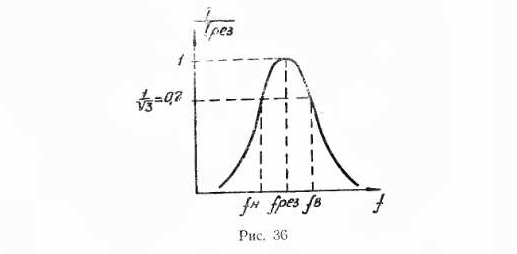
\includegraphics[scale=0.85]{ekon3_032_1}

В конструкторе в качестве колебательного контура используется магнитная антенна. При приёме сигналов близко расположенных радиостанций внешнюю антенну можно не использовать.

Следует иметь в виду, что громкость приёма зависит от направленности магнитной антенны на передающую радиостанцию.

При сборке приёмников необходимо учесть, что уверенный приём сигналов радиовещательных станций зависит от многих факторов: удалённости от передающих стнаций, уровня помех в месте приёма, степени разряда источника питания, наличия внешней антенны. Поэтому при отсутствии местных 

\newpage

радиостанций, удалённость которых от места приёма не более 30 км, приёмники могут работать недостаточно качественно.

Для увеличения дальности приёма необходимо использовать внешние комантные или наружные антенны.

Устройство комнатной антенны приведено в приложении 3.
\vspace*{1cm}
\subsubsection{Радиоприёмник 2-V-1}

На рис.37 представлена схема радиоприёмника 2-V-1. Это означает, что радиоприёмник имеет два каскада усления высокой частоты, детектор и один каскад усиления низкой частоты. В качестве усилителя высокой частоты (УВЧ) используется микросхема, причем  первый её транзистор включен по схеме с общим эмиттером, второй - по схеме с общим коллектором, т.е. в качестве эмиттерного повторителя. Такой УВЧ менее склонен к самовозбуждению и хорошо согласуется с детектором.

\vspace*{0.5cm}
\hrulefill

\begin{tabular}{r l r p{0.5cm} r l r p{0.5cm} r l r p{0.5cm} r l r}
14 - & 21  & - К &     & 34 - & 37      &   - К    &      &  49 - & 112 & - K &     &  71 - & 108 & - С\\
15 - & 67  & - К &     & 34 - & 44      &   - С    &      &  50 - & 113 & - K &     &  76 - & 116 & - К\\
16 - & 57  & - K &     & 35 - & 36      &   - К    &      &  52 - &  56 & - K &     &  77 - & 109 & - С\\
17 - & 53  & - C &     & 36 - & 99      &   - K    &      &  53 - &  69 & - К &     &  98 - & 123 & - К\\
18 - & 123 & - С &     & 37 - & 64      &   - С    &      &  62 - & 114 & - К &     & 113 - & 116 & - К\\
19 - & 23  & - K &     & 38 - & 98      &   - К    &      &  63 - &  66 & - К &     & 116 - & 123 & - С\\
21 - & 77  & - С &     & 47 - & 111     &   - К    &      &  65 - &  77 & - К &     & 117 - & 46  & - Д\\
21 - & 117 & - С &     & 48 - & 110     &   - К    &      &  66 - &  68 & - К &     & 118 - & 124 & - К\\
24 - & 114 & - С &     & 49 - & 55      &   - К    &      &  68 - & 116 & - К &     &       &     &    \\
33 - & 108 & - С &     & 54 - & \mc{2}{c}{антенна} &      &  70 - & 115 & - С &     &       &     &    \\
\end{tabular}

\hrulefill

\vspace*{1cm}
\subsubsection{Радиоприёмник 2-V-2}

Усилитель высокой частоты приёмника, схема которого изображена на рис.38, аналогичен УВЧ на рис.37. Трансформатор Т1 служит для согласования УВЧ с детектором. Усилитель низкой частоты радиоприёмника собран на двух транзисторах разной структуры (n-p-n и p-n-p). Такое включение транзисторов позволяет уменьшить количество переходных конденсаторов.

\newpage

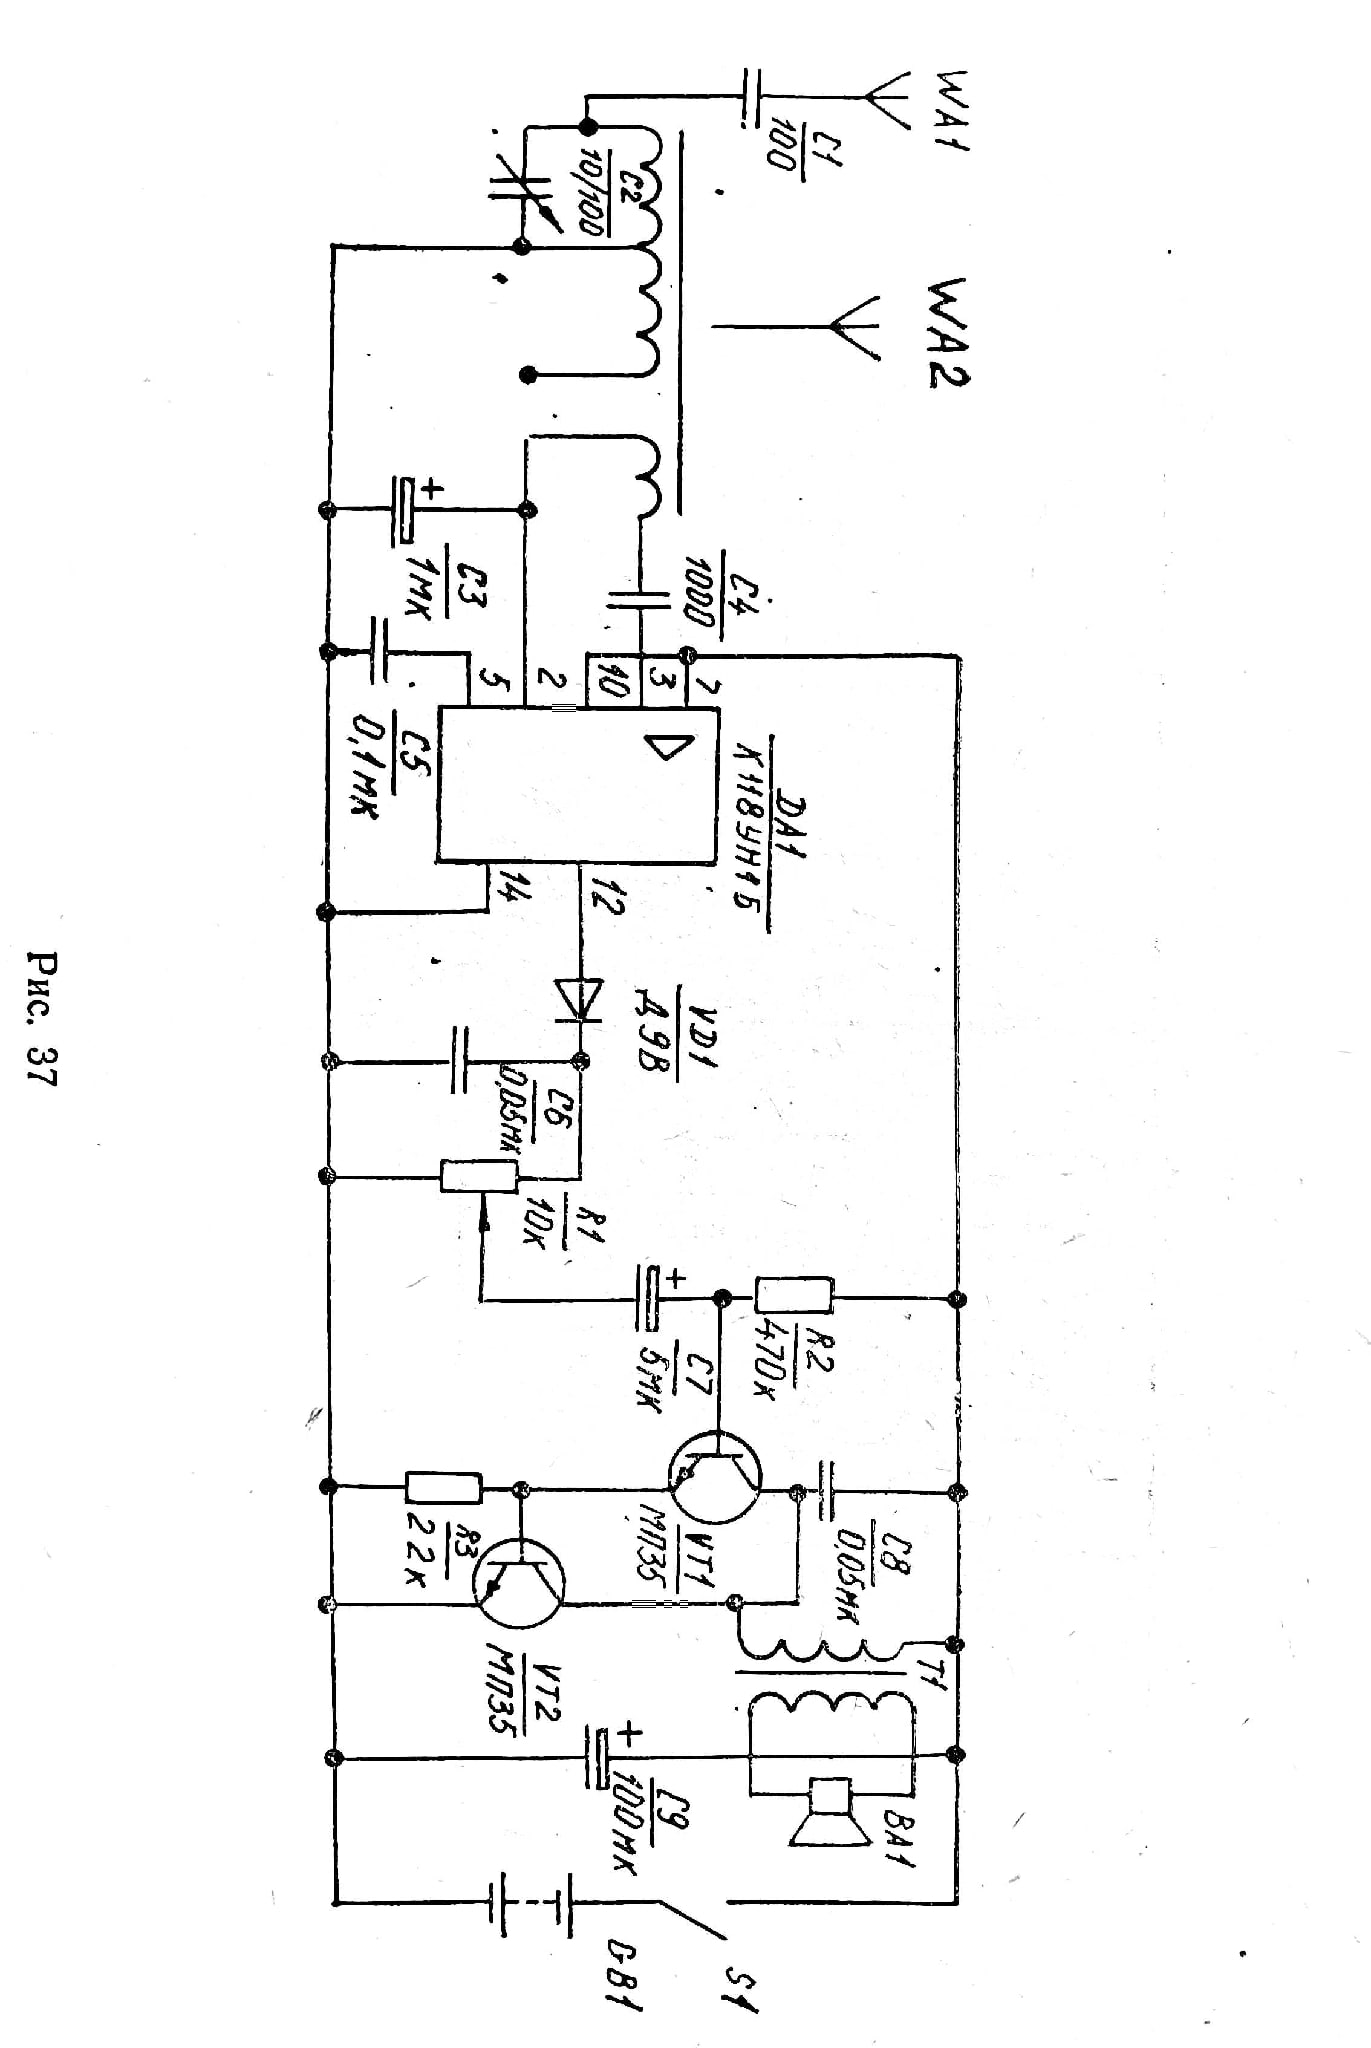
\includegraphics[scale=0.35, angle=180]{Fig37}

\newpage

\vspace*{1cm}
\hspace*{0.7cm}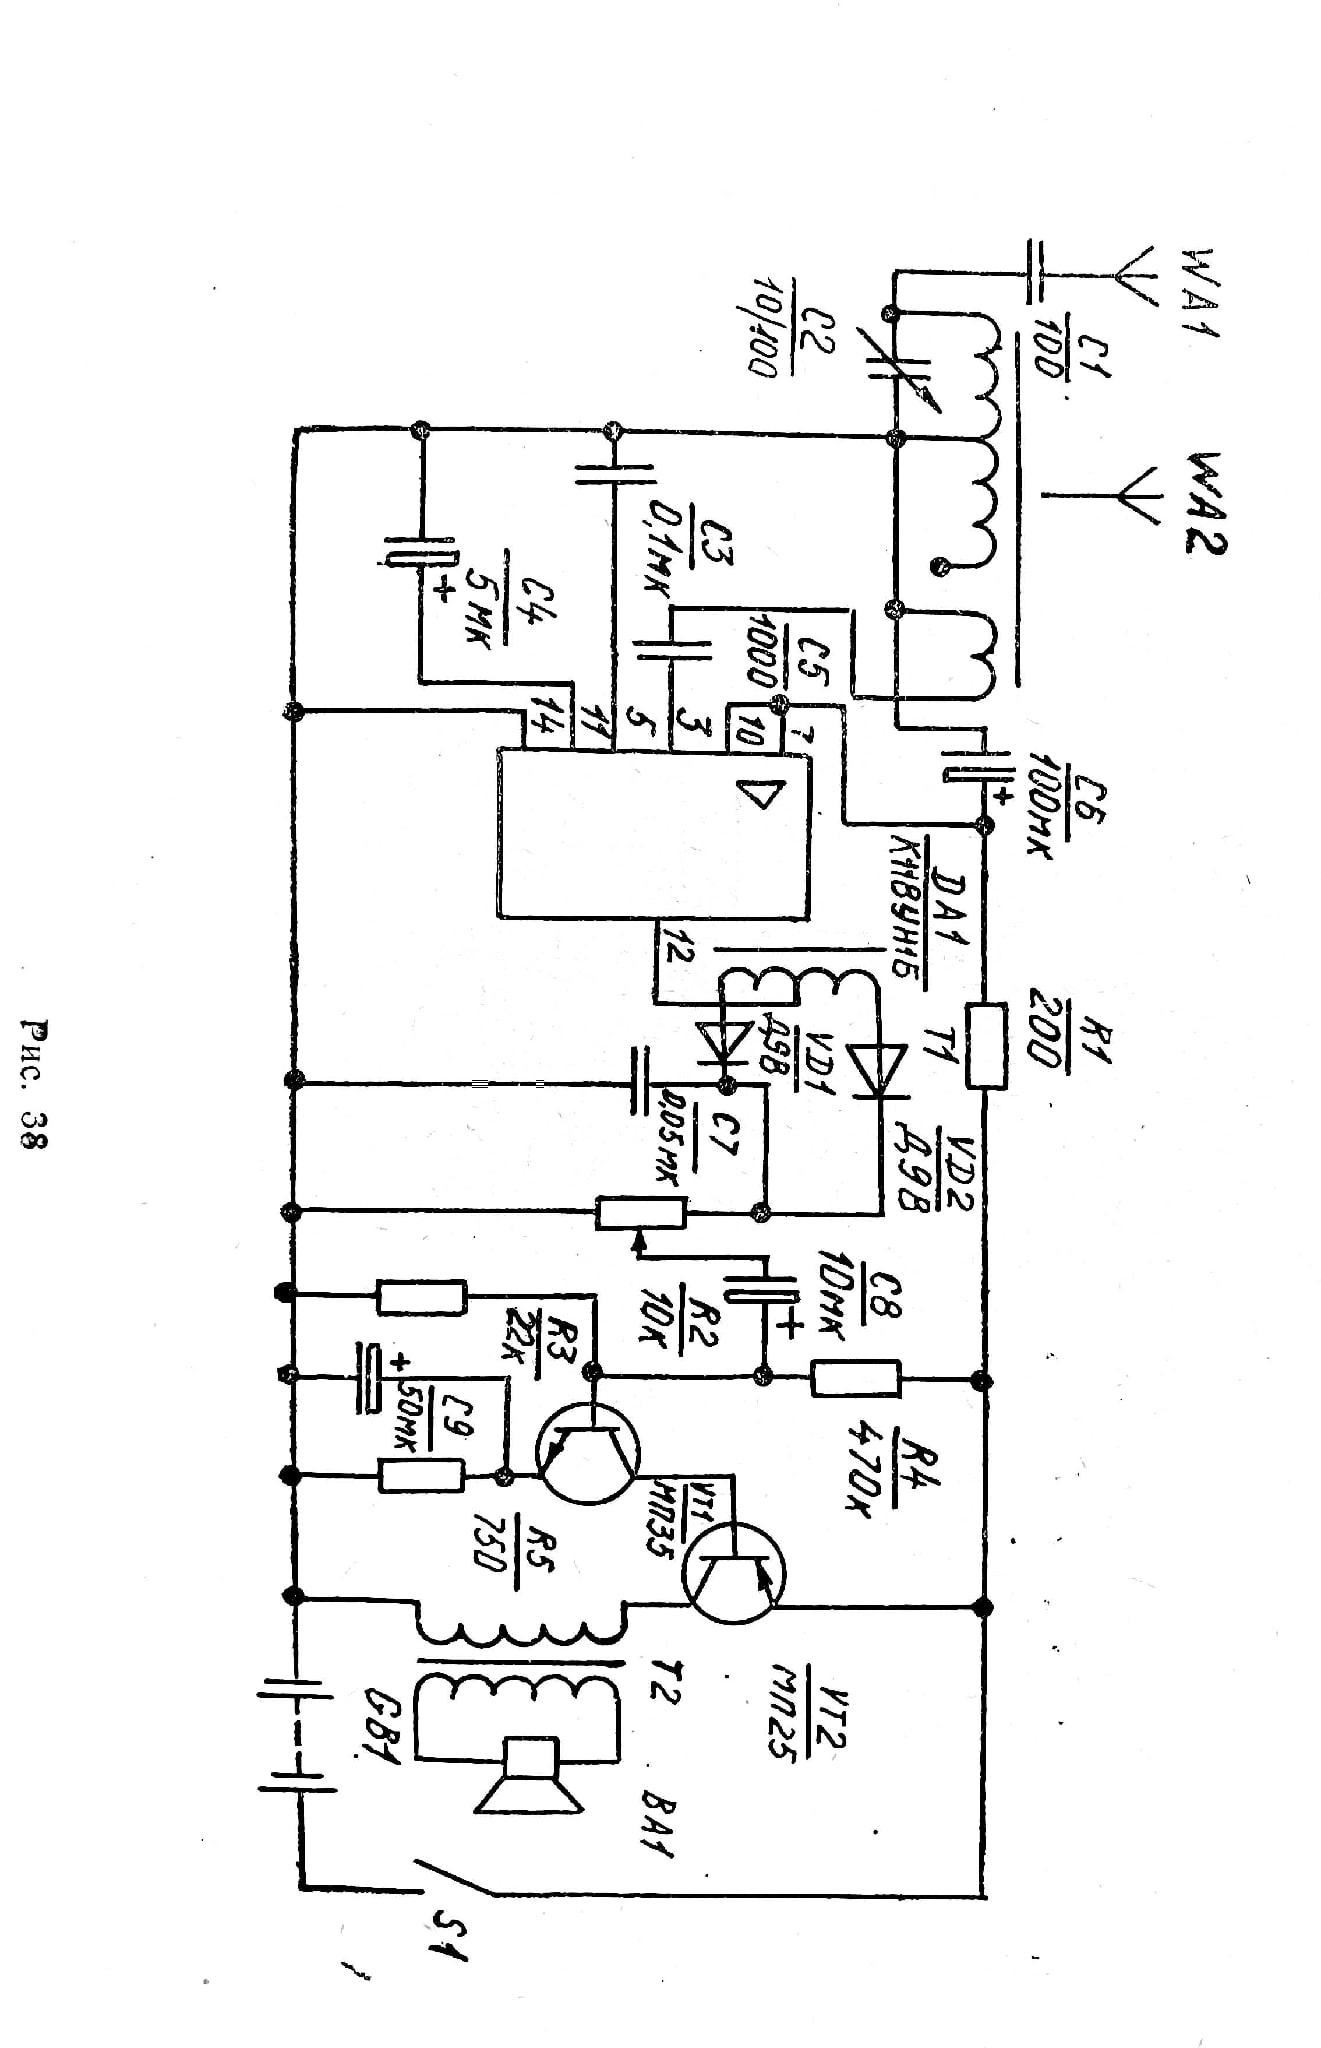
\includegraphics[scale=0.35, angle=180]{Fig38}

\newpage

\hrulefill

\begin{tabular}{r l r p{0.5cm} r l r p{0.5cm} r l r p{0.5cm} r l r}
14 - & 21  & - К &     & 27 - & 31      &   - К    &      &  49 - & 112 & - K &     &  75 - &  87 & - С\\
14 - & 77  & - К &     & 28 - & 44      &   - С    &      &  50 - &  53 & - K &     &  77 - &  82 & - К\\
15 - & 67  & - K &     & 29 - & 108     &   - C    &      &  50 - & 113 & - K &     &  83 - & 117 & - К\\
16 - & 57  & - К &     & 30 - & 73      &   - K    &      &  52 - &  56 & - К &     &  83 - & 108 & - К\\
18 - & 70  & - К &     & 30 - & 109     &   - С    &      &  64 - & 114 & - К &     &  86 - &  98 & - К\\
19 - & 40  & - С &     & 32 - & 87      &   - К    &      &  65 - & 116 & - К &     &  98 - & 116 & - С\\
20 - & 71  & - К &     & 46 - & 123     &   - C    &      &  66 - &  76 & - К &     &  98 - & 123 & - К\\
23 - & 41  & - С &     & 47 - & 111     &   - К    &      &  66 - & 116 & - К &     &  99 - & 109 & - К\\
24 - & 26  & - К &     & 48 - & 110     &   - К    &      &  66 - &  70 & - К &     & 113 - & 116 & - К\\
24 - & 114 & - С &     & 49 - & 55      &   - K    &      &  72 - & 115 & - К &     & 118 - & 124 & - К\\
25 - & 39  & - С &     & 54 - & \mc{2}{c}{антенна} &      &  74 - &  76 & - К &     &       &     &    \\
\end{tabular}

\hrulefill

\vspace*{2cm}
\subsubsection{Радиоприёмник 2-V-4}
\vspace*{1cm}
В радиоприёмнике, схема которого изображена на рис. 39, усилители высокой и низкой частоты собраны с использованием микросхемы, а усилитель мощности выполнен по бестрансформаторной схеме.

    
\hrulefill

\begin{tabular}{r l r p{0.5cm} r l r p{0.5cm} r l r p{0.5cm} r l r}
 5 - & 12  & - К &     & 25 - & 29     &   - К    &      &  49 - &  55 & - K &         &  73 - & 106 & - С\\
 6 - & 69  & - С &     & 26 - & 37     &   - С    &      &  49 - & 113 & - K &         &  74 - & 116 & - К\\
 7 - & 57  & - K &     & 27 - & 73     &   - C    &      &  50 - &  53 & - K &         &  75 - &  82 & - К\\
 9 - & 18  & - К &     & 28 - & 36     &   - K    &      &  50 - & 112 & - К &         &  77 - & 110 & - Д\\
 9 - & 70  & - К &     & 28 - & 60     &   - Д    &      &  52 - &  56 & - К &         &  83 - &  89 & - К\\
10 - & 23  & - К &     & 29 - & 61     &   - Д    &      &  62 - &  72 & - К &         &  83 - & 117 & - К\\
12 - & 82  & - С &     & 29 - & 76     &   - C    &      &  63 - &  74 & - К &         &  84 - & 116 & - С\\
14 - & 21  & - К &     & 29 - & 35     &   - К    &      &  54 - &  \mc{2}{c}{антенна} & &  84 - & 123 & - К\\
15 - & 71  & - К &     & 33 - & 88     &   - С    &      &  63 - &  68 & - К &         & 107 - & 123 & - К\\
16 - & 67  & - К &     & 33 - & 37     &   - K    &      &  64 - & 114 & - К &         & 111 - & 117 & - Д\\
19 - & 72  & - С &     & 34 - & 89     &   - С    &      &  65 - &  70 & - К &         & 112 - & 116 &   К\\
21 - & 83  & - К &     & 36 - & 85     &   - С    &      &  66 - & 115 & - К &         & 118 - & 124 & - К\\
24 - & 114 & - С &     & 38 - & 107    &   - K    &      &  70 - & 116 & - К &         &       &     &    \\
\end{tabular}

\hrulefill

\newpage
\hspace*{0.7cm}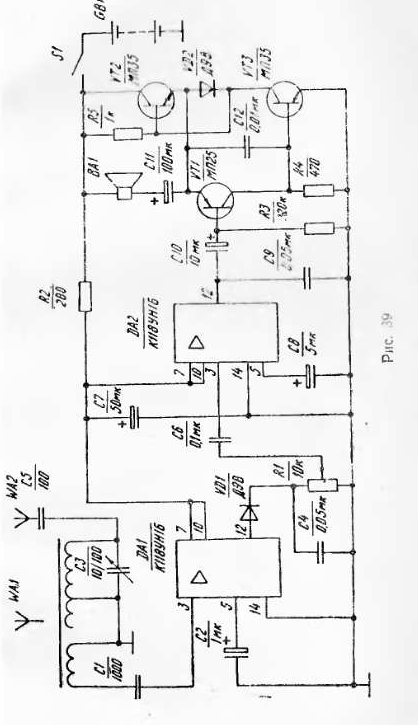
\includegraphics[scale=0.99, angle=-1]{ekon3_037_1}

\newpage

\subsubsection{Радиоприёмник 2-V-4}
УВЧ приёмника, схема которого изображена на рис. 40, не отличается от применённой в предыдущем приёмнике. В усилителе низкой частоты используются трансформаторы.

\hrulefill

\begin{tabular}{r l r p{0.5cm} r l r p{0.5cm} r l r p{0.5cm} r l r}
 5 - & 12  & - К &     & 30 - & 91     &   - К    &      &  45 - & 117 & - Д          &     &  70 - & 116 & - К\\
 6 - & 71  & - К &     & 31 - & 42     &   - К    &      &  47 - & 111 & - С          &     &  72 - &  90 & - С\\
 7 - & 57  & - K &     & 32 - & 79     &   - К    &      &  48 - & 110 & - K          &     &  74 - &  76 & - К\\
 9 - & 18  & - К &     & 33 - & 39     &   - K    &      &  49 - &  55 & - К          &     &  74 - &  79 & - К\\
10 - & 23  & - К &     & 34 - & 46     &   - С    &      &  49 - & 112 & - К          &     &  74 - & 123 & - С\\
12 - & 21  & - К &     & 35 - & 38     &   - К    &      &  50 - &  53 & - К          &     &  76 - & 116 & - К\\
14 - & 21  & - К &     & 35 - & 78     &   - С    &      &  50 - & 113 & - К          &     &  77 - &  84 & - К\\
14 - & 77  & - К &     & 35 - & 110    &   - С    &      &  52 - &  56 & - К          &     &  85 - & 107 & - К\\
15 - & 75  & - К &     & 36 - & 41     &   - С    &      &  63 - &  65 & - К          &     &  85 - & 117 & - К\\
16 - & 94  & - С &     & 37 - & 44     &   - С    &      &  64 - & 114 & - К          &     &  91 - & 106 & - К\\
18 - & 76  & - С &     & 40 - & 93     &   - С    &      &  65 - &  70 & - К          &     &  92 - & 111 & - С\\
19 - & 62  & - С &     & 40 - & 99     &   - С    &      &  54 - & \mc{2}{c}{антенна} &     & 113 - & 116 & - К\\
19 - & 73  & - С &     & 43 - & 107    &   - K    &      &  68 - &  95 & - С          &     & 118 - & 124 & - K\\
24 - & 114 & - С &     & 45 - & 98     &   - С    &      &  69 - & 115 & - К          &     &       &     &    \\
\end{tabular}

\hrulefill

\subsubsection{Радиоприёмник 2-V-3}

Радиоприёмник, схема которого изображена на рис.41, отличается от предыдущих усилителем низкой частоты. Транзистор VT2 осуществляет температурную стабилизацию усилителя.

\newpage

\hspace*{2.7cm}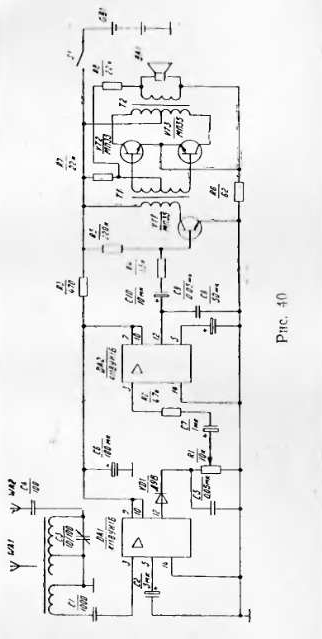
\includegraphics[scale=1.1, angle=0]{ekon3_039_1}

\newpage

\hspace*{0.7cm}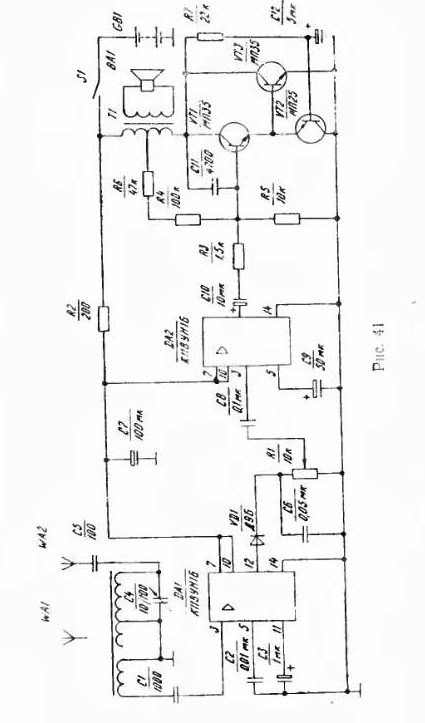
\includegraphics[scale=0.99, angle=-1]{ekon3_040_1}

\newpage

\hrulefill

\begin{tabular}{r l r p{0.5cm} r l r p{0.5cm} r l r p{0.5cm} r l r}
 5 - & 12  & - К &     & 24 - & 114 & - С &      &  45 - & 100 & - С          &     &  68 - & 116 & - К\\
 6 - & 61  & - С &     & 27 - &  71 & - С &      &  47 - & 111 & - К          &     &  70 - &  74 & - К\\
 7 - & 57  & - K &     & 27 - & 102 & - К &      &  48 - & 110 & - K          &     &  72 - &  90 & - С\\
 9 - & 18  & - К &     & 28 - &  38 & - K &      &  49 - &  55 & - К          &     &  74 - & 116 & - К\\
 9 - & 76  & - С &     & 28 - &  96 & - С &      &  54 - & \mc{2}{c}{антенна} &     &  74 - &  76 & - К\\
10 - & 23  & - К &     & 29 - &  36 & - К &      &  49 - & 112 & - К          &     &  77 - &  82 & - К\\
11 - & 69  & - С &     & 33 - &  91 & - С &      &  50 - &  52 & - К          &     &  83 - & 117 & - К\\
12 - & 21  & - К &     & 33 - &  59 & - Д &      &  50 - & 113 & - К          &     &  91 - & 104 & - К\\
12 - & 82  & - С &     & 34 - &  46 & - С &      &  53 - &  56 & - К          &     &  96 - & 123 & - К\\
14 - & 21  & - К &     & 34 - &  37 & - К &      &  58 - & 103 & - Д          &     &  97 - & 104 & - К\\
15 - & 75  & - С &     & 35 - &  36 & - К &      &  60 - &  68 & - К          &     & 101 - & 105 & - К\\
16 - & 67  & - С &     & 37 - & 103 & - С &      &  64 - &  68 & - К          &     & 113 - & 116 & - К\\
19 - & 73  & - С &     & 44 - &  83 & - С &      &  65 - & 114 & - К          &     & 116 - & 123 & - С\\
     &     &     &     &      &     &     &      &  66 - & 115 & - К          &     & 118 - & 124 & - С\\
\end{tabular}

\hrulefill

\subsubsection{Радиоприёмник 2-V-2}

В радиоприёмнике, схема которого изображена на рис. 42, использован усилитель низкой частоты с двухтактным трансформаторным выходным каскадом, а УВЧ выполнен на микросхеме.

\newpage

\hspace*{0.7cm}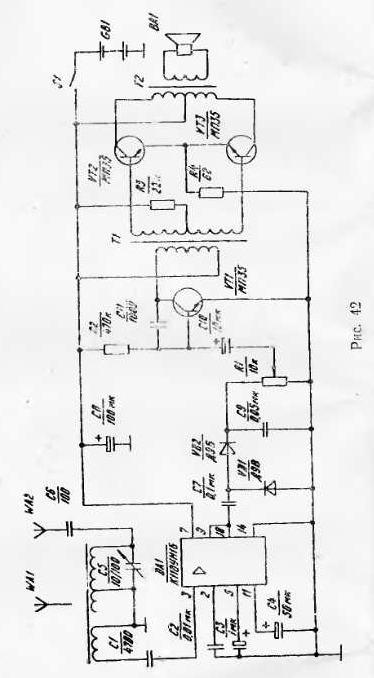
\includegraphics[scale=0.99, angle=-1]{ekon3_042_1}

\newpage

\hrulefill

\begin{tabular}{r l r p{0.5cm} r l r p{0.5cm} r l r p{0.5cm} r l r}
 5 - & 77  & - C &     & 30 - & 109 & - С &      &  47 - & 111 & - К          &     &  68 - & 113 & - К\\
 6 - & 69  & - С &     & 31 - &  42 & - К &      &  48 - & 110 & - К          &     &  72 - & 115 & - К\\
 7 - & 59  & - K &     & 31 - &  56 & - С &      &  49 - &  55 & - K          &     &  76 - & 116 & - К\\
 8 - & 60  & - C &     & 32 - &  78 & - K &      &  49 - & 112 & - К          &     &  77 - & 108 & - С\\
 9 - & 116 & - С &     & 33 - &  39 & - К &      &  50 - &  52 & - К          &     &  78 - & 123 & - С\\
11 - & 75  & - C &     & 34 - &  46 & - С &      &  50 - & 113 & - К          &     &  99 - & 117 & - К\\
12 - & 13  & - K &     & 35 - &  38 & - К &      &  53 - &  58 & - К          &     & 113 - & 116 & - К\\
12 - & 66  & - К &     & 35 - &  79 & - С &      &  54 - & \mc{2}{c}{антенна} &     & 116 - & 123 & - С\\
23 - & 26  & - K &     & 36 - &  41 & - К &      &  57 - &  73 & - К          &     & 108 - & 117 & - К\\
23 - & 67  & - C &     & 37 - &  44 & - С &      &  61 - & 113 & - К          &     & 118 - & 124 & - К\\
24 - & 64  & - С &     & 40 - &  98 & - С &      &  64 - & 114 & - К          &     &       &     &   \\
25 - & 65  & - K &     & 43 - & 117 & - С &      &  65 - &  68 & - К          &     &       &     &   \\
30 - & 73  & - С &     & 45 - &  99 & - С &      &  68 - &  74 & - К          &     &       &     &   \\
\end{tabular}

\hrulefill

\subsection{АВТОМАТИЧЕСКИЕ УСТРОЙСТВА}

\subsubsection{Триггер Шмитта}

В схеме (рис. 43) оба транзистора связаны по постоянному току через резистор сопротивлением 1,5 кОм и резистор сопротивлением 470 Ом в цепи эмиттеров. В качестве нагрузки второго каскада служит светодиод. На базу первого транзистора с потенциометра подаётся напряжение, которое можно изменять.

\hspace*{0.7cm}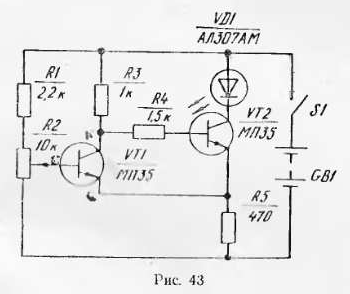
\includegraphics[scale=0.99, angle=1]{ekon3_043_1}

\newpage

\hrulefill

\begin{tabular}{r c r c r p{2cm} r c r c r p{2cm} r c r c r}
32 & - &  38 & - & К &     & 89  & - & 90 & - & К &    & 116 & - & 84  & - & К\\
84 & - & 123 & - & К &     & 91  & - & 36 & - & С &    & 117 & - & 119 & - & K\\
85 & - &  32 & - & K &     & 93  & - & 88 & - & К &    & 118 & - & 124 & - & С\\
88 & - & 117 & - & K &     & 114 & - & 30 & - & C &    & 120 & - &  37 & - & С\\
89 & - &  31 & - & K &     & 115 & - & 92 & - & C &    &     &   &     &   &  \\
\end{tabular}

\hrulefill

Ось потенциометра устанавливают в левое крайнее положение. Напряжение на базе первого транзистора равно нулю. Ток коллектора отсутствует. На первом транзисторе падает практически полностью напряжение питания, которое подаётся на базу второго транзистора. Оно достаточно для полного открывания второго транзистора, о чём свидетельствует свечение светодиода. Ось потенциометра медленно вращают вправо. Сначала никаких изменений в работе схемы не происходит. При определённом положении оси потенциометра светодиод мгновенно гаснет.

Через резистор сопротивлением 470 Ом осуществляется взаимосвязь между транзисторами. Благодаря этой взаимосвязи происходит скачкообразное изменение состояния устройства. При этом первый транзистор полностью открывается, а второй оказывается закрытым. Если же теперь ось потенциометра вращать в обратном направлении, то при определённом её положении светодиод мгновенно загорится.

Примечание: если бы эмиттер VT1 был бы подключен на <<->> питания, тогда эта схема работала бы просто как усилитель постоянного тока, без триггерного эффекта и без гистерезиса.

\subsubsection{Триггер Шмитта с усилительным каскадом}

Через резистор сопротивлением 22 кОм базу транзистора усилительного каскада подключают к триггеру Шмитта (рис.44). Светодиод включён в цепь коллектора усилительного каскада.

\newpage

\hspace*{0.7cm}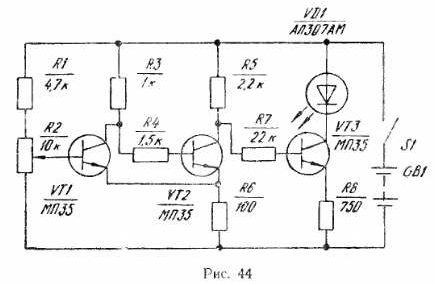
\includegraphics[scale=0.99, angle=0]{ekon3_045_1}

\hrulefill

\begin{tabular}{r c r c r p{2cm} r c r c r p{2cm} r c r c r}
32 & - &  38 & - & К &     & 88  & - & 92  & - & К &    &  95 & - &  88 & - & К\\
32 & - &  80 & - & К &     & 89  & - & 31  & - & К &    &  99 & - &  33 & - & С\\
37 & - &  98 & - & C &     & 90  & - & 89  & - & С &    & 114 & - &  94 & - & С\\
81 & - &  87 & - & K &     & 91  & - & 36  & - & C &    & 115 & - &  30 & - & С\\
86 & - &  35 & - & K &     & 92  & - & 119 & - & К &    & 116 & - & 123 & - & С\\
87 & - & 116 & - & C &     & 93  & - & 37  & - & C &    & 117 & - & 119 & - & К\\
   &   &     &   &   &     & 120 & - & 34  & - & C &    & 118 & - & 124 & - & С\\
\end{tabular}

\hrulefill

В отличие от предыдущего устройства, светодиод включается, когда возрастает положительное напряжение на базе первого транзистора, и гаснет, когда напряжение на ней понижается.

\subsubsection{Фоторезистор - регулирующий элемент в триггере Шмитта}

Схема (рис.45) представляет собой триггер Шмитта с дополнительным каскадом. На входе триггера стоит фоторезистор. При закрытом окне фоторезистора светодиод не горит. Откройте окно фоторезистора. Светодиод загорится почти мгновенно. Это происходит оттого, что напряжение на входе триггера стало выше напряжения переключения.

Сесли светодиод не горит, осветите окно фоторезистора каким-либо дополнительным источником света (фонарик, настольная лампа и т.д.).

\newpage
\hspace*{0.7cm}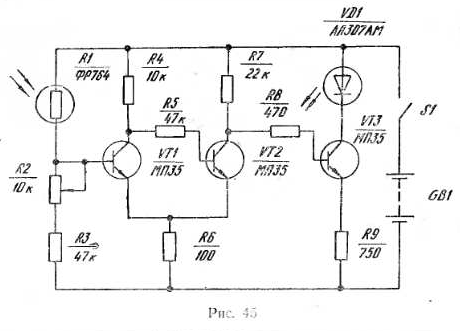
\includegraphics[scale=0.99, angle=0]{ekon3_046_1}

\hrulefill

\begin{tabular}{r l r p{0.5cm} r l r p{0.5cm} r l r p{0.5cm} r l r}
30 - & 121 & - C &   & 36 - & 101 & - С &   & 85 - &  33 & - С &   &  98 - &  37 & - С\\
32 - &  38 & - К &   & 81 - &  86 & - К &   & 96 - &  31 & - К &   &  99 - & 119 & - К\\
32 - &  80 & - K &   & 81 - & 123 & - К &   & 96 - & 100 & - K &   & 119 - & 124 & - К\\
35 - &  87 & - К &   & 84 - &  98 & - K &   & 97 - &  99 & - К &   & 120 - &  34 & - С\\
     &     &     &   & 30 - &  88 & - К &   & 89 - & 123 & - К &   & 124 - & 122 & - К\\
\end{tabular}

\hrulefill

\subsubsection{Индикатор влажности}

По принципу работы схема (рис. 46) аналогична предыдущей. В качестве датчика влажности используется два электрода, которые можно изготовить из отрезков проволоки длиной 100-150 мм.

При контроле влажности, например, земли в цветочном горшке электроды помещают в цветочный горшок с сухой землёй и соединяют их со схемой. Ось переменного резистора следует установить в такое положение , при котором светодиод (при неподключенных проводах) начинает гаснуть. Если наливать воду в цветочный горшок, то при определённой влажности земли светодиод загорится.

\newpage
\hspace*{0.7cm}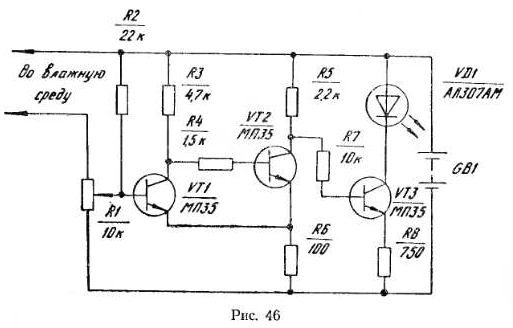
\includegraphics[scale=0.9, angle=0]{ekon3_047_1}

\hrulefill

\begin{tabular}{r l r p{0.5cm} r l r p{0.5cm} r l r p{0.5cm} r l r}
30 - &  98 & - К &   & 34 - & 120 & - С &   & 81 - & 116 & - К &   &  93 - &  99  & - С\\
30 - & 115 & - С &   & 35 - &  87 & - К &   & 81 - & 123 & - К &   &  93 - & 119  & - К\\
31 - &  94 & - K &   & 36 - &  91 & - К &   & 90 - &  94 & - K &   &  99 - & \mc{2}{l}{вход} \\
32 - &  38 & - К &   & 37 - &  92 & - С &   & 92 - &  96 & - К &   & 114 - & \mc{2}{l}{вход} \\
32 - &  80 & - К &   & 81 - &  86 & - К &   & 93 - &  95 & - К &   & 119 - & 124  & - К\\
33 - &  97 & - С &   &      &     &     &   &      &     &     &   &       &      &    \\
\end{tabular}

\hrulefill

\subsubsection{Мультивибратор}

Мультивибратор представляет собой генератор электрических колебаний, близких к прямоугольной форме.

\hspace*{0.7cm}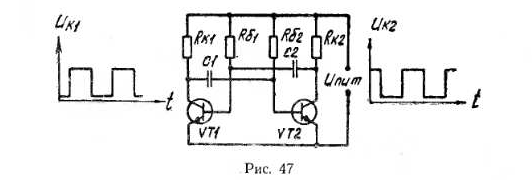
\includegraphics[scale=0.9, angle=0]{ekon3_047_2}

Схема, изображённая на рис. 47, представляет собой два усилительных каскада. Транзистор VT1, его нагрузочный ре-

\newpage
зистор $R_{\text{к1}}$ и базовый $R_{\text{б1}}$ образуют первый каскад, а тразистор VT2 и резисторы $R_{\text{к2}}$ и $R_{\text{б2}}$ - второй.

Выход первого каскада через конденсатор C1 связан со входом второго, а выход второго каскада - через конденсатор C2 - со входом первого. Благодаря такой взаимосвязи двухкаскадное устройство становится мультивибратором.

На рис.47 изображены графики напряжений на коллекторах транзисторов. Видно, что транзисторы каждого плеча мультивибратора работают в режиме переключения. Любой транзистор поочерёдно бывает в открытом и закрытом состояниях. Причём, если один из них открыт, другой - закрыт, т.е. транзисторы работают со сдвигом фазы на 180\textdegree.

Соберите мультивибратор согласно схеме рис.48.

\hspace*{0.7cm}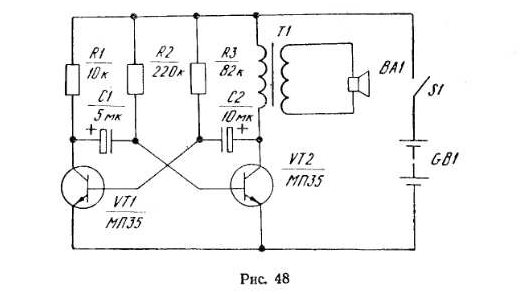
\includegraphics[scale=0.9, angle=0]{ekon3_048_1}

\hrulefill

\begin{tabular}{r c r c r p{2cm} r c r c r p{2cm} r c r c r}
30 & - &  72 & - & C &     & 48  & - & 110 & - & К &    &  96 & - & 106 & - & К\\
32 & - &  38 & - & К &     & 70  & - & 107 & - & С &    & 102 & - &  44 & - & С\\
36 & - &  70 & - & C &     & 71  & - &  31 & - & С &    & 106 & - & 102 & - & К\\
37 & - &  46 & - & C &     & 71  & - &  97 & - & C &    & 106 & - & 118 & - & К\\
38 & - & 123 & - & C &     & 72  & - & 103 & - & С &    & 117 & - & 124 & - & С\\
47 & - & 111 & - & К &     & 73  & - &  37 & - & C &    &     &   &     &   &  \\
\end{tabular}

\hrulefill

Подключив мультивибратор  итксчонику питания, можно услышать в громкоговорителе сигнал определённой частоты. Частота генерируемых мультивибратором колебаний зависит от величины сопротивлений резисторов в цепях коллекторов и баз транзисторов, а также от ёмкости конденсаторов. Частоту колебаний симметричного мультивибратора (симметричным называется 

\newpage
такой мультивибратор, у которого номиналы элементов, образующих плечи, попарно равны) можно приближённо подсчитать по формуле

\begin{equation}
f = \frac{1}{RC}
\end{equation}

где f - частота, Гц\\
R - сопротивление резистора, Ом\\
C - ёмкость конденсатра, Ф

Пользуясь этой формулой, подсчитайте, колебания каких частот генерировали ваши мультивибраторы.

\subsubsection{Мультивибратор с переменной частотой колебаний}

Замените постоянный резистор в цепи коллектора левого транзистора регулируемым резистором (рис. 49). При вращении оси региулруемого резистора изменяется высота звука.

\hspace*{0.7cm}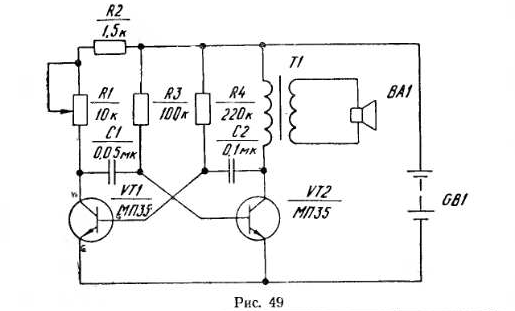
\includegraphics[scale=0.9, angle=0]{ekon3_049_1}

\hrulefill

\begin{tabular}{r c r c r p{2cm} r c r c r p{2cm} r c r c r}
32 & - &  38 & - & К &     &  64 & - & 114 & - & К &    & 105 & - &  36 & - & К\\
38 & - & 123 & - & С &     &  65 & - &  36 & - & С &    & 106 & - &  44 & - & С\\
46 & - &  37 & - & C &     &  66 & - &  30 & - & С &    & 106 & - & 124 & - & К\\
47 & - & 111 & - & К &     &  67 & - &  37 & - & C &    & 107 & - &  30 & - & С\\
48 & - & 110 & - & К &     &  91 & - & 104 & - & К &    & 115 & - & 116 & - & К\\
64 & - &  31 & - & С &     & 104 & - & 106 & - & К &    & 116 & - &  90 & - & С\\
\end{tabular}

\hrulefill

\newpage

\subsubsection{Ждущий мультивибратор}

Ждущий мультивибратор имеет одно устойчивое состояние , в котором может находиться до тех пор, пока поданный на вход старотовыйим пульс не выведет его в другое, неустойчивое состояние. Длительность импульса,в ырабатываемого ждущи ммуьтливибратормо, не зависит от длительности стартового импульса, а определяется лишь величинами сопротивлений резисторов и ёмкостями конденсаторов, входящих в схему, поэтому светодиод горит ещё некоторое время после отпускания ключа (рис.50).

\hspace*{0.7cm}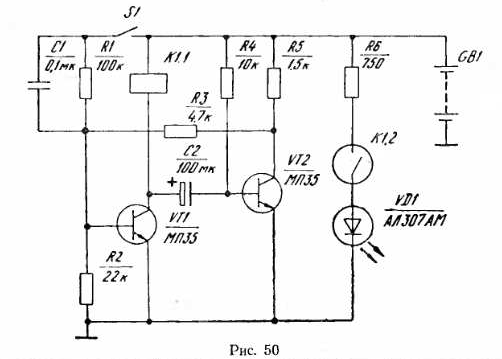
\includegraphics[scale=0.9, angle=0]{ekon3_050_1}

\hrulefill

\begin{tabular}{r l r p{0.5cm} r l r p{0.5cm} r l r p{0.5cm} r l r}
 1 - &  31 & - С &   & 32 - & 38 & - К &   & 66 - & 104 & - С &   &  94 - & 104  & - С\\
 2 - &  96 & - С &   & 32 - & 99 & - К &   & 67 - & 105 & - С &   &  99 - & 123  & - К\\
 3 - & 119 & - Д &   & 36 - & 76 & - С &   & 87 - & 124 & - С &   & 120 - & 123  & - K\\
 4 - &  86 & - С &   & 36 - & 97 & - К &   & 91 - &  96 & - К &   & 124 - & 125  & - К\\
30 - &  98 & - К &   & 37 - & 90 & - С &   & 91 - & 124 & - С &   & 105 - & 126  & - С\\
31 - &  77 & - С &   & 37 - & 95 & - К &   & 94 - &  98 & - К &   &       &      &    \\
\end{tabular}

\hrulefill

\subsubsection{Электронный коммутатор}
При прикосновении к проводу <<Вход>> загорается светодиод. Время его горения определяется параметрами ждущего 

\newpage

мультивибратора. Данное устройство можно использвтоаь в качестве электронного коммутатора, замыкающего электрическую цепь на определённый промжеутк овремени. Схема электрическая электронного коммутатора приведена на рис.51

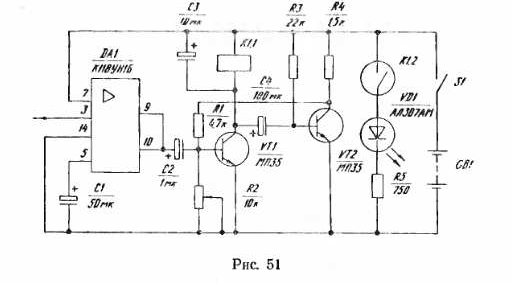
\includegraphics[scale=1, angle=0]{ekon3_051_1}

\hrulefill

\begin{tabular}{r l r p{0.5cm} r l r p{0.5cm} r l r p{0.5cm} r l r}
 1 - &  14 & - С &   & 21 - & 22 & - К &   & 36 - &  97 & - К &   &  91 - & 124  & - К\\
 2 - &  31 & - С &   & 22 - &100 & - С &   & 37 - &  94 & - К &   &  92 - & 123  & - К\\
 3 - & 119 & - Д &   & 30 - & 93 & - С &   & 74 - &  92 & - С &   &  93 - & 101  & - K\\
 4 - &  14 & - К &   & 31 - & 77 & - С &   & 86 - & 120 & - К &   &  95 - & 101  & - К\\
14 - &  96 & - С &   & 32 - & 38 & - К &   & 87 - &  74 & - С &   &  16 - & \mc{2}{l}{вход} \\
15 - &  75 & - С &   & 32 - & 92 & - К &   & 90 - &  94 & - К &   &       &      &    \\
18 - &  74 & - С &   & 36 - & 76 & - С &   & 91 - &  96 & - К &   &       &      &    \\
\end{tabular}

\hrulefill

\newpage

\subsubsection{Устройство подачи светового сигнала}

Нагрузкой правого плеча мультивибратора является реле, попеременно включающее и выклюающее светодиод (рис. 52).

\includegraphics[scale=1, angle=1]{ekon3_052_1}

\hrulefill

\begin{tabular}{r c r c r p{2cm} r c r c r p{2cm} r c r c r}
 1 & - &  37 & - & Д &     &  31 & - &  75 & - & С &    &  37 & - &  77 & - & С\\
 2 & - &  96 & - & С &     &  31 & - &  92 & - & С &    &  87 & - & 124 & - & С\\
 3 & - & 119 & - & Д &     &  32 & - & 123 & - & С &    &  93 & - &  98 & - & К\\
 4 & - &  86 & - & С &     &  32 & - &  38 & - & К &    &  93 & - & 124 & - & К\\
30 & - &  76 & - & С &     &  36 & - &  99 & - & К &    &  96 & - &  98 & - & К\\
30 & - &  97 & - & К &     &  36 & - &  74 & - & С &    & 120 & - & 123 & - & К\\
\end{tabular}

\hrulefill

\subsubsection{Генератор с эмиттерной связью}

Этот генератор (рис.53) можно назвать генератором со стопроцентной обратной связью по току. Работает он как пороговое устройство. При определённом положении оси регулируемого резистора генератор возбуждается, и в громкоговорителе слышен звук.

\newpage

\includegraphics[scale=1, angle=1]{ekon3_053_1}

\hrulefill

\begin{tabular}{r l r p{0.5cm} r l r p{0.5cm} r l r p{0.5cm} r l r}
30 - &  95 & - К &   & 33 - & 71 & - С &   & 37 - &  43 & - К &   &  88 - & 117  & - К\\
31 - &  36 & - К &   & 33 - & 91 & - С &   & 37 - & 116 & - Д &   &  90 - & 117  & - К\\
32 - &  38 & - К &   & 34 - & 46 & - С &   & 44 - & 124 & - С &   &  94 - & 114  & - K\\
32 - &  70 & - С &   & 35 - &117 & - С &   & 47 - & 111 & - К &   & 115 - & 116  & - К\\
32 - &  89 & - К &   & 36 - & 42 & - К &   & 48 - & 110 & - К &   & 116 - & 124  & - C\\
     &     &     &   &      &    &     &   &      &     &     &   & 118 - & 123  & - К\\
\end{tabular}

\hrulefill

\subsubsection{Генератор колебаний на микросхеме}

На рис. 54 изображена схема генератора, в котором обратная связь с выхода на вход осуществляется за счёт конденсатора ёмкостью 0,1 мкФ. Если необходимо получить колебания другой частоты, нужно изменить ёмкость конденсатора связи. При использовании конденсатора большей ёмкости частота колебаний уменьшается.

\newpage

\includegraphics[scale=1, angle=0]{ekon3_054_1}

\hrulefill

\begin{tabular}{r c r c r p{2cm} r c r c r p{2cm} r c r c r}
 14 & - &  46 & - & Д &     &  18 & - & 123 & - & С &    &  47 & - & 111 & - & К\\
 14 & - & 117 & - & С &     &  21 & - &  66 & - & С &    &  48 & - & 110 & - & К\\
 15 & - &  67 & - & К &     &  21 & - &  44 & - & С &    & 118 & - & 124 & - & К\\
\end{tabular}

\hrulefill

Сигнал обратной связи может быть подан на другой вход схемы (рис.55)

\vspace*{0.3cm}
\includegraphics[scale=1, angle=0]{ekon3_054_2}

\newpage

\hrulefill

\begin{tabular}{r c r c r p{2cm} r c r c r p{2cm} r c r c r}
 14 & - &  46 & - & Д &     &  18 & - & 123 & - & С &    &  47 & - & 111 & - & К\\
 14 & - & 117 & - & С &     &  21 & - &  66 & - & С &    &  48 & - & 110 & - & К\\
 16 & - &  67 & - & К &     &  21 & - &  44 & - & С &    & 118 & - & 124 & - & К\\
\end{tabular}

\hrulefill

\subsubsection{Индикатор внешней освещённости со звуковой индикацией}

На микросхеме построен генератор низкочастотных колебаний (рис.56). При хорошей освещённости фоторезистора его сопротивление уменьшается, генерация колебаний исчезает. Звук отсутствует. При понижении освещённости возникают НЧ-колебания, которые усиливаются однокаскадным усилителем на транзисторе и воспроизводятся в виде звукового сигнала громкоговорителем.

\includegraphics[scale=1, angle=0]{ekon3_055_1}

\newpage

\hrulefill

\begin{tabular}{r c r c r p{2cm} r c r c r p{2cm} r c r c r}
 14 & - &  46 & - & Д &     &  22 & - &  71 & - & К &    &  46 & - & 124 & - & С\\
 16 & - &  66 & - & С &     &  30 & - &  70 & - & К &    &  47 & - & 111 & - & К\\
 16 & - & 122 & - & Д &     &  30 & - &  96 & - & К &    &  48 & - & 110 & - & К\\
 18 & - &  32 & - & С &     &  31 & - &  44 & - & С &    & 118 & - & 123 & - & К\\
 21 & - &  22 & - & К &     &  31 & - &  97 & - & К &    & 124 & - & 121 & - & К\\
 21 & - &  67 & - & С &     &  32 & - & 117 & - & С &    &     &   &     &   &  \\
\end{tabular}

\hrulefill

\subsubsection{ Индикатор внешней освещённости со световой индикацией}

Левая часть схемы аналогична изображённой на рис.55. НЧ-сигнал, снятый со вторичной обмотки трансформатора, детектируется диодом. Постоянное напряжение, являющееся результатом детектирования, управляет усилителем, собранным на правом транзисторе (рис. 57).
Его нагрузкой является светодиод, который загорится при понижении освещённости.

\newpage

\includegraphics[scale=1.25, angle=1]{ekon3_057_1}

\newpage

\hrulefill

\begin{tabular}{r l r p{0.5cm} r l r p{0.5cm} r l r p{0.5cm} r l r}
14 - & 118 & - C &   & 24 - & 78 & - К &   & 32 - &  99 & - К &   &  78 - &  98  & - К\\
16 - &  62 & - К &   & 30 - & 68 & - С &   & 36 - &  79 & - К &   &  86 - &  99  & - К\\
16 - & 121 & - Д &   & 30 - &100 & - С &   & 37 - & 120 & - С &   &  99 - & 123  & - K\\
18 - &  32 & - С &   & 31 - & 42 & - К &   & 38 - &  87 & - К &   &  63 - &  69  & - К\\
21 - &  22 & - К &   & 31 - &101 & - С &   & 43 - & 122 & - С &   & 117 - & 124  & - C\\
22 - &  63 & - К &   & 32 - & 39 & - К &   & 43 - & 118 & - С &   & 119 - & 118  & - К\\
23 - &  41 & - С &   &      &    &     &   &      &     &     &   &       &      &    \\
\end{tabular}

\hrulefill

\subsubsection{ Имитатор щебетания птиц }
Этот генератор является имитатором щебетания птиц. Изменяя освещённость фоторезистора, можно увеличивать или уменьшать частоту колебаний генератора. В схему включена цепочка, состоящая из последвательно соединённых резисторов сопротивлением 1 кОм и электролитического конденсатора ёмкостью 100 мкФ (рис.58).

В период заряда конденсатор не оказывает влияния на работу генератора. Разряжается он через участок база-эмиттер транзистора. Отрицательное напряжение на базе во время разряда увеличивается, транзистор закрывается, и срывается генерация.

\includegraphics[scale=0.9, angle=0]{ekon3_058_1}

\newpage

Полностью разрядившись, конденсатор начинает снова заряжаться, первоначальное напряжение на базе восстанавливается, транзистор открывается, и схема генерирует колебания.

\hrulefill

\begin{tabular}{r c r c r p{2cm} r c r c r p{2cm} r c r c r}
 31 & - &  62 & - & С &     &  63 & - &  67 & - & К &    &  89 & - &  66 & - & С\\
 32 & - &  76 & - & С &     &  67 & - &  44 & - & Д &    &  89 & - & 121 & - & С\\
 46 & - &  31 & - & С &     &  76 & - & 117 & - & К &    & 118 & - & 123 & - & К\\
 47 & - & 111 & - & К &     &  77 & - &  88 & - & К &    & 124 & - &  45 & - & С\\
 48 & - & 110 & - & К &     &  89 & - &  30 & - & К &    & 124 & - & 122 & - & К\\
\end{tabular}

\hrulefill

\subsubsection{Электронный <<Маяк>>}

На микросхеме выполнен генератор очень низкой частоты (рис. 59).Т ранзистор является усилителем постоянного тока. <<Мигание>> начинается через несколько секунд после включения схемы.


\includegraphics[scale=0.9, angle=0]{ekon3_059_1}

\hrulefill

\begin{tabular}{r c r c r p{2cm} r c r c r p{2cm} r c r c r}
 14 & - &  86 & - & К &     &  76 & - &  16 & - & К &    & 119 & - &  28 & - & С\\
 18 & - & 117 & - & С &     &  77 & - &  21 & - & К &    & 120 & - & 123 & - & К\\
 22 & - &  21 & - & К &     &  81 & - &  22 & - & К &    & 124 & - &  14 & - & С\\
 27 & - &  80 & - & К &     &  86 & - & 124 & - & С &    &     &   &     &   &  \\
 29 & - &  87 & - & К &     & 118 & - & 123 & - & С &    &     &   &     &   &  \\
\end{tabular}

\hrulefill

\newpage

\subsubsection{ Генератор с непосредственной связью между транзисторами}

В этой схеме два транзистора непосредственно соединены друг с другом, что даёт возможность собрать простой генератор с достаточно болоьшйв ыходной мощностью. Частоту  колебаний в небольших пределах можно изменять, изменяя величину сопротивления переменного резистора (рис. 60).

\includegraphics[scale=0.9, angle=0]{ekon3_060_1}

\hrulefill

\begin{tabular}{r l r p{0.5cm} r l r p{0.5cm} r l r p{0.5cm} r l r}
27 - &  31 & - К &   & 29 - & 114 & - Д &   &  32 - & 110 & - С &   & 110 - & 118  & - Д\\
28 - &  81 & - С &   & 30 - &  66 & - С &   &  67 - &  80 & - К &   & 114 - & 124  & - С\\
28 - & 111 & - С &   & 30 - & 104 & - К &   & 116 - & 105 & - С &   & 115 - & 116  & - K\\
     &     &     &   &      &     &     &   &       &     &     &   & 117 - & 123  & - К\\
\end{tabular}

\hrulefill

\subsubsection{ Звуковой <<Маяк>>}

На микросхеме, изображенной слева (рис. 61), выполнен генератор очень низкой частоты. Он управляет работой генератора, собранного на микросхеме (справа) через транзистор, используемый в качестве ключа.

\newpage

\includegraphics[scale=1, angle=0]{ekon3_061_1}

\vspace*{5.5cm}

\hrulefill

\begin{tabular}{r l r p{0.5cm} r l r p{0.5cm} r l r p{0.5cm} r l r}
 5 - & 101 & - C &   & 13 - &  77 & - С &   &  21 - &  22 & - К &   &  44 - & 101  & - С\\
 7 - &  76 & - С &   & 14 - &  38 & - С &   &  22 - &  70 & - К &   &  47 - & 110  & - К\\
 9 - &  18 & - К &   & 16 - &  62 & - К &   &  30 - &  71 & - К &   &  48 - & 111  & - K\\
12 - &  13 & - К &   & 18 - &  32 & - С &   &  30 - & 100 & - К &   &  63 - &  70  & - К\\
13 - &  36 & - С &   & 18 - & 117 & - С &   &  31 - &  46 & - С &   & 101 - & 124  & - К\\
     &     &     &   &      &     &     &   &  37 - &  44 & - К &   & 118 - & 123  & - К\\
\end{tabular}

\hrulefill

\subsubsection{Генератор нестандартных сигналов}
Схема (рис. 62) состоит из двух мульивибраторов. Средий транзистор входит и в первый, и во второй мультивибратор. 

\newpage

Благодаря этому, при нажатии на ключ получается весьма интересный звуковой эффект.

\includegraphics[scale=1, angle=0]{ekon3_062_1}

\hrulefill

\begin{tabular}{r l r p{0.5cm} r l r p{0.5cm} r l r p{0.5cm} r l r}
30 - &  62 & - C &   & 35 - &  81 & - С &   &  48 - & 111 & - К &   &  84 - & 126  & - С\\
30 - & 102 & - К &   & 36 - &  72 & - С &   &  63 - &  66 & - К &   &  85 - & 123  & - К\\
31 - &  88 & - К &   & 36 - & 105 & - К &   &  64 - &  88 & - С &   &  89 - & 117  & - K\\
32 - &  79 & - К &   & 37 - &  44 & - К &   &  65 - &  72 & - К &   &  89 - & 103  & - К\\
33 - &  67 & - С &   & 37 - &  63 & - С &   &  73 - &  90 & - К &   &  89 - & 106  & - К\\
33 - & 107 & - С &   & 38 - &  78 & - С &   &  78 - &  80 & - К &   &  95 - & 106  & - К\\
34 - &  90 & - С &   & 46 - & 103 & - С &   &  80 - &  91 & - К &   & 103 - & 104  & - К\\
34 - &  94 & - К &   & 47 - & 110 & - К &   &  84 - &  91 & - К &   & 118 - & 124  & - К\\
     &     &     &   &      &     &     &   &       &     &     &   & 123 - & 125  & - С\\
\end{tabular}

\hrulefill

\subsubsection{ Генератор с затухающими колебаниями}

Конденсаторы обладают свойством накапливать электрическую энергию. Чем больше ёмкость конднесатора, тем больше он может накопить энергии, которая потом постепенно расходуется (рис.63).

\newpage

В данной схеме при нажатии на ключ батарея питания подключается к схеме блокинг-генератора, и в грокоговорителе слышен звук. При отпускании ключа звук слышен с затуханием ещё некоторое время, так как блокинг-генератор продолжае тработать за счёт энергии, накопленной электролитическим конденсатором.

\includegraphics[scale=1, angle=1]{ekon3_063_1}

\vspace{5cm}

\hrulefill

\begin{tabular}{r l r p{0.5cm} r l r p{0.5cm} r l r p{0.5cm} r l r}
30 - &  42 & - C &   & 37 - &  46 & - С &   &  47 - & 111 & - К &   &  81 - & 102  & - К\\
31 - &  39 & - К &   & 38 - & 123 & - С &   &  48 - & 110 & - К &   &  81 - & 126  & - С\\
31 - &  69 & - С &   & 41 - &  80 & - С &   &  62 - &  69 & - К &   & 105 - & 117  & - С\\
32 - &  38 & - К &   & 43 - & 103 & - К &   &  63 - & 103 & - С &   & 118 - & 124  & - К\\
36 - &  68 & - С &   & 44 - & 105 & - С &   &  76 - & 123 & - С &   &       &      &    \\
36 - & 104 & - К &   & 44 - & 125 & - С &   &  77 - &  81 & - К &   &       &      &    \\
\end{tabular}

\hrulefill

\newpage

\subsubsection{Индикатор освещённости}

При освещении фоторезистора его сопротивление уменьшается, вследствие чего увеличивается ток через транзисторы, реле срабатывает, а светодиод включается (рис.64).

\includegraphics[scale=1, angle=0]{ekon3_064_1}

\vspace{6cm}

\hrulefill

\begin{tabular}{r c r c r p{2cm} r c r c r p{2cm} r c r c r}
 1 & - & 124 & - & Д &     & 33 & - & 121 & - & C &    &  38 & - & 123  & - & C\\
 2 & - &  37 & - & Д &     & 34 & - & 122 & - & С &    &  87 & - & 124  & - & С\\
 3 & - & 119 & - & Д &     & 35 & - &  85 & - & C &    & 120 & - & 123  & - & К\\
 4 & - &  86 & - & C &     & 36 & - &  84 & - & С &    & 122 & - & 124  & - & К\\
\end{tabular}

\hrulefill

\newpage

\subsubsection{Мультивибратор на микросхемах}

Принцип работы этого мультивибратора аналогичен принципу работы транзисторного, но в каждом его плече вместо транзистора используется микросхема (рис.65).

\includegraphics[scale=1, angle=0]{ekon3_065_1}

\hrulefill

\begin{tabular}{r c r c r p{2cm} r c r c r p{2cm} r c r c r}
 5 & - &  14 & - & К &     & 14 & - & 117 & - & C &    &  22 & - &  46  & - & Д\\
 7 & - &  64 & - & С &     & 16 & - &  63 & - & К &    &  47 & - & 111  & - & К\\
 9 & - &  18 & - & К &     & 18 & - & 123 & - & C &    &  48 & - & 110  & - & К\\
12 & - &  13 & - & К &     & 21 & - &  44 & - & С &    & 118 & - & 124  & - & К\\
12 & - &  62 & - & К &     & 21 & - &  65 & - & С &    &     &   &      &   &  \\
\end{tabular}

\hrulefill

\subsubsection{Электронный генератор}

Регулируемый резистор (рис.66) позволяет изменять частоту следования импульсов. Генератор может быть использован в качестве дверного звонка.

\newpage


\includegraphics[scale=1, angle=0]{ekon3_066_1}

\hrulefill

\begin{tabular}{r c r c r p{2cm} r c r c r p{2cm} r c r c r}
27 & - &  31 & - & К &     & 29 & - & 124 & - & C &    &  75 & - & 116  & - & К\\
28 & - &  68 & - & С &     & 30 & - &  69 & - & С &    &  88 & - & 114  & - & С\\
28 & - &  81 & - & С &     & 30 & - &  89 & - & К &    & 114 & - & 115  & - & К\\
28 & - & 110 & - & С &     & 32 & - &  74 & - & С &    & 117 & - & 123  & - & К\\
29 & - &  75 & - & С &     & 32 & - &  80 & - & К &    & 118 & - & 111  & - & С\\
\end{tabular}

\hrulefill

\subsubsection{ <<Электромузыкальный инструмент>>}

Изменяя освещённость фоторезистора (например, прикрывая его окно рукой), можно изменять частоту колебаний генератора (рис.67).

\hrulefill

\begin{tabular}{r l r p{0.5cm} r l r p{0.5cm} r l r p{0.5cm} r l r}
 5 - &  14 & - К &   & 13 - &  63 & - К &   &  22 - &  70 & - К &   &  47 - & 111  & - К\\
 6 - & 122 & - Д &   & 14 - & 101 & - С &   &  30 - &  71 & - К &   &  48 - & 110  & - К\\
 7 - &  62 & - К &   & 16 - &  73 & - К &   &  30 - & 100 & - С &   &  69 - &  73  & - К\\
 9 - &  18 & - К &   & 18 - &  32 & - С &   &  31 - &  44 & - С &   & 101 - & 117  & - К\\
12 - &  13 & - К &   & 21 - &  22 & - К &   &  32 - & 123 & - С &   & 117 - & 121  & - С\\
12 - &  72 & - К &   & 21 - &  68 & - С &   &  46 - & 101 & - С &   & 118 - & 124  & - К\\
\end{tabular}

\hrulefill

\newpage

\includegraphics[scale=1, angle=-0.5]{ekon3_067_1}

\newpage

\subsubsection{Индикатор влажности}

Этот прибор служит для определения влажности (рис.68). Если электроды попадают во влажную среду, чеерз неё замыкается цепь обратной связи, возникает генерация НЧ-колебаний, которые воспрзвоиодятся громкоговорителем.

\includegraphics[scale=1, angle=-0.5]{ekon3_068_1}

\hrulefill

\begin{tabular}{r l r p{0.5cm} r l r p{0.5cm} r l r p{0.5cm} r l r}
16   & \multicolumn{2}{l}{ во влаж-} &   & 21 - &  22 & - К &   &  31 - &  44 & - С &   &  48 - & 110  & - К\\
62   & \multicolumn{2}{l}{ную среду} &   & 22 - &  63 & - К &   &  32 - & 123 & - С &   &  63 - &  74  & - К\\
14 - & 101 & - C                     &   & 30 - &  75 & - С &   &  46 - & 101 & - С &   & 101 - & 117  & - К\\
18 - &  32 & - C                     &   & 30 - & 100 & - С &   &  47 - & 111 & - К &   & 118 - & 124  & - К\\
\end{tabular}

\hrulefill

\subsubsection{ Индикатор сильных звуков}

Принцип работы этого устройства (рис.69) аналогичен изображенному на рис. 57. Громкоговоритель используется в качестве микрофона. Если перед ним произносить звуки достаточной громкости, загорается светодиод.

\hrulefill

\begin{tabular}{r l r p{0.5cm} r l r p{0.5cm} r l r p{0.5cm} r l r}
 1 - &  14 & - К &   & 22 - &  71 & - К &   &  32 - &  38 & - К &   &  48 - & 110  & - К\\
 2 - &  37 & - Д &   & 25 - &  43 & - С &   &  32 - &  93 & - К &   &  76 - &  93  & - С\\
 3 - &  88 & - C &   & 26 - &  85 & - К &   &  36 - &  84 & - С &   &  77 - &  92  & - С\\
 4 - & 119 & - C &   & 30 - &  70 & - С &   &  38 - & 123 & - С &   &  85 - &  92  & - К\\
14 - &  39 & - C &   & 30 - &  94 & - К &   &  39 - & 117 & - Д &   &  89 - & 124  & - К\\
16 - &  72 & - К &   & 31 - &  41 & - С &   &  42 - &  44 & - К &   & 118 - & 124  & - С\\
18 - &  32 & - C &   & 31 - &  95 & - К &   &  46 - &  73 & - Д &   & 120 - & 123  & - К\\
21 - &  22 & - К &   & 32 - &  42 & - К &   &  47 - & 111 & - К &   &       &      &    \\
\end{tabular}

\hrulefill

\newpage

\includegraphics[scale=1, angle=0]{ekon3_069_1}

\newpage

\subsubsection{Регулятор напряжения}

В данной схеме в качестве регулирующего выходное напряжение элемента используется транзистор (рис. 70). Подобные схемы используются очень широко, когда необходимо регулировать большие токи, и в схеамх стабилизаторов напряжения. Если между верхним по схеме выводом потенциометра и общим выводом 14 микросхемы установить стабилитрон (элемент, поддерживающий постоянное напряжение независимо от сопротивления нагрузки), можно получить сехму параметрического стабилизатора, напряжение на выходе котороог не изменяется под действием изменяющегося сопротивления нагрузки (тока в нагрузке).

\vspace{1cm}

\includegraphics[scale=1, angle=0]{ekon3_070_1}

\vspace{1cm}

\hrulefill

\begin{tabular}{r c r c r p{2cm} r c r c r p{2cm} r c r c r}
14 & - &  31 & - & С &     & 31 & - &  34 & - & К &    &  84 & - & 119  & - & К\\
14 & - &  99 & - & С &     & 32 & - &  36 & - & К &    &  98 & - & 114  & - & С\\
16 & - & 115 & - & С &     & 33 & - &  36 & - & К &    &  99 & - & 117  & - & К\\
18 & - & 116 & - & С &     & 34 & - &  37 & - & К &    & 116 & - & 123  & - & С\\
21 & - &  22 & - & К &     & 35 & - &  38 & - & К &    & 118 & - & 124  & - & К\\
22 & - &  30 & - & К &     & 38 & - &  85 & - & С &    & 120 & - & 123  & - & К\\
\end{tabular}

\hrulefill

\newpage

\subsubsection{Генератор пилообразного напряжения}

На трёх n-p-n транзисторах собран генератор пилообразного напряжения, частоту колебаний которого можно изменять при помощи потенциометра. Этим напряжением через эмиттерный повторитель, выполненный на p-n-p-транзисторе, питается генератор низкочастотных колебаний на изображенной слева микросхеме. Микросхема, изображенная справа, выполняет роль усилителя низкой частоты. При работе схемы в громкоговорителе слышен постепенно изменяющийся по частоте сигнал. Эта схема изображена на рис. 71.

\hrulefill

\begin{tabular}{r l r p{0.5cm} r l r p{0.5cm} r l r p{0.5cm} r l r}
 5 - &  14 & - К &   & 18 - &  68 & - С &   &  32 - &  35 & - К &   &  91 - & 123  & - К\\
 7 - &  62 & - К &   & 20 - &  69 & - С &   &  33 - & 115 & - Д &   &  93 - & 100  & - К\\
 9 - &  29 & - C &   & 21 - &  44 & - С &   &  34 - &  38 & - К &   &  93 - & 117  & - К\\
12 - &  13 & - К &   & 27 - &  94 & - К &   &  34 - &  95 & - К &   &  96 - & 104  & - К\\
12 - &  63 & - К &   & 28 - &  32 & - К &   &  37 - &  73 & - С &   & 100 - & 104  & - К\\
13 - &  66 & - К &   & 28 - &  70 & - С &   &  38 - &  77 & - С &   & 101 - & 116  & - С\\
14 - &  93 & - C &   & 30 - &  72 & - С &   &  70 - &  76 & - К &   & 104 - &  46  & - С\\
15 - &  71 & - К &   & 30 - & 105 & - С &   &  73 - &  92 & - К &   & 110 - &  48  & - К\\
16 - &  67 & - C &   & 31 - &  36 & - К &   &  76 - &  91 & - С &   & 111 - &  47  & - К\\
18 - &  28 & - С &   & 31 - &  97 & - К &   &  90 - & 114 & - С &   & 118 - & 124  & - К\\
\end{tabular}

\hrulefill

\newpage

\includegraphics[scale=0.8, angle=0]{ekon3_072_1}

\newpage

\subsubsection{Блокинг-генератор}

Блокинг-генератор выполнен на транзисторе, изображенном слева. Необходимая для возникновения генерации обратная связь осуществляется за счёт трансформатора. С помощью переменного резистора можно изменять частоту генерируемых колебаний. На транзисторе, изображенном справа, выполнен усилитель (рис. 72).

\vspace{1.5cm}

\includegraphics[scale=1, angle=0]{ekon3_073_1}

\vspace{1.5cm}

\hrulefill

\begin{tabular}{r c r c r p{2cm} r c r c r p{2cm} r c r c r}
 23 & - &  31 & - & К &     &  31 & - &  42 & - & К &    &  43 & - &  46 & - & К\\
 23 & - &  98 & - & С &     &  32 & - &  38 & - & К &    &  47 & - & 111 & - & К\\
 24 & - &  43 & - & С &     &  36 & - &  99 & - & К &    &  48 & - & 110 & - & К\\
 24 & - & 114 & - & С &     &  37 & - &  44 & - & К &    &  96 & - & 115 & - & С\\
 30 & - &  39 & - & С &     &  38 & - & 123 & - & С &    & 114 & - & 117 & - & С\\
    &   &     &   &   &     &  41 & - &  97 & - & С &    & 118 & - & 124 & - & К\\
\end{tabular}

\hrulefill

\newpage

\subsubsection{Сторожевое устройство с проволочной петлёй}

Эта схема представляет собой сигнальное устройство, в которомбаз а транзистора замкнута на эмиттер с помощью провоолчной петли. Эту петлю можно выполнить из длинного тонкого провода, проустив её, например, через двери и окна охраняемого помещения. При разрыве провода ликвидируется замыкани ецепи базы транзистора и возникает сигналт ревоги. Эмиттер транзистора подключен к <<+>> батареи GB1. Схема устройства представлена на рис. 73.

\vspace{1.5cm}

\includegraphics[scale=1, angle=0]{ekon3_074_1}

\vspace{1.5cm}

\hrulefill

\begin{tabular}{r c r c r p{2cm} r c r c r p{2cm} r c r c r}
 1 & - & 123 & - & Д &     &  27 & - &  29 & - & петля &    &  86 & - & 119 & - & С\\
 2 & - &  28 & - & С &     &  27 & - &  95 & - & К     &    &  87 & - & 124 & - & С\\
 3 & - & 120 & - & Д &     &  29 & - & 124 & - & С     &    &  94 & - & 123 & - & С\\
 4 & - &  94 & - & С &     &     &   &     &   &       &    &     &   &     &   &  \\
\end{tabular}

\hrulefill

\newpage

\subsubsection{Аварийная сирена}

В этой схеме (рис. 74) генератор, собранный на микросхеме, изображенной слева, управляет работой звукового генератора и светодиода. Через некоторые промежутки времени одновременно вырабатываются звуковой и световой сигналы, дающие эффект работы аварийной сирены.

\vspace{1.5cm}

\includegraphics[scale=1, angle=0]{ekon3_075_1}

\vspace{1.5cm}

\hrulefill

\begin{tabular}{r l r p{0.5cm} r l r p{0.5cm} r l r p{0.5cm} r l r}
 1 - &  12 & - К &   &  9 - &  18 & - К &   &  21 - &  46 & - Д &   &  71 - &  73  & - К\\
 2 - &   5 & - К &   & 10 - &  70 & - К &   &  21 - &  63 & - К &   &  73 - & 117  & - К\\
 3 - & 119 & - Д &   & 12 - &  14 & - К &   &  22 - &  44 & - С &   &  74 - &  76  & - К\\
 4 - &  86 & - С &   & 12 - &  75 & - С &   &  47 - & 111 & - К &   &  75 - &  77  & - К\\
 5 - &  71 & - К &   & 16 - &  62 & - К &   &  48 - & 110 & - К &   &  87 - & 124  & - С\\
 7 - &  74 & - С &   & 18 - & 123 & - С &   &  70 - &  72 & - К &   & 118 - & 124  & - К\\
     &     &     &   &      &     &     &   &       &     &     &   & 120 - & 123  & - К\\
\end{tabular}

\hrulefill

\part{ПРИЛОЖЕНИЕ 3}

\section{УСТРОЙСТВО КОМНАТНОЙ АНТЕННЫ}

Наиболее простой для самостоятельного изготовления является комнатная антенна. Она состоит из горизонтального провода 1 длиной 2-4 м, укреплённого с помощью изоляторов 2 на высоте около 2 м от пола; вертикального провода 3, называемого синжением (рис. 75).

В качестве горизонтального провода и снижения могут быть использованы антенный канатик, монтажный или обмоточный провод. В качестве изоляторов можно применить отрезки пластмассы.

\includegraphics[scale=1, angle=0]{ekon3_076_1}

На схемах электрических принципиальных внешняя антенна обозначается так, как показано на рис.76.

\includegraphics[scale=1, angle=0]{ekon3_076_2}

\newpage

\section{ЛИТЕРАТУРА}

\begin{itemize}
\item[1] Богданович Б. М., Ваксер Э. Б. Краткий радиотехнический справочник. Минск, <<Беларусь>>, 1968.
\item[2] Булыч В. И. Юному конструктору. М., ДОСААФ, 1977.
\item[3] Бурлянд В. А., Жеребцов И. П. Хрестоматия радиолюбителя. М., <<Энергия>>? 1971.
\item[4] Тихонов С.Н. Радиотехника для начинающих. М., Воениздат, 1976.
\item[5] В помощь радиолюбителю. Вып. 39, 1972.
\item[6] Гершунский Б.С. Основы электроники. Киев, <<Вища школа>>, 1971.
\item[7] Горшков А.П. Как установить радиоприёмник. М., ГИЛ по вопрсоам связи и радио, 1958.
\item[8] Дзюбин  И. И., Енин А . А. Путешествие в мир раидоэлектроники. М., <<Просвящение>>, 1980
\item[9] Загорский Я.Т. и др. Измерительные усилители на транзисторах. М., <<Энергия>>, 1971.
\item[10] Лосев А.К. Введение в  специальность <<Радиотехника>>. М., <<Высшая школа>>, 1980
\item[11] Мамезлев И.А., Капелин Г.Г. Основы радиоэлектроники. М., <<Просвящение>>, 1980.
\item[12] Начинающим радиолюбителям. Ж. <<Радио>>, 1975
\item[13] Справочник по транзисторным схемам. Под ред. Р. М. Малинина Изд. 2-е. Массовая радиобиблиотека. Вып. 852, М., <<Энергия>>, 1974.
\end{itemize}

\newpage


\tableofcontents

\end{document}